\documentclass[10pt]{report}

%%%%%%%%%%%%%%%%%%%%%%%%%%%%%%%%%% DEBUT DU PREAMBULE %%%%%%%%%%%%%%%%%%%%%%%%%%%%%%%%%
\title{Rapport Devoir ARA}															%%%
\usepackage[francais]{babel}														%%%
\usepackage[T1]{fontenc}															%%%
\usepackage[utf8]{inputenc}															%%%
\usepackage{fancyhdr}																%%%
\usepackage{lastpage}																%%%
\usepackage{graphicx, wrapfig, subcaption, setspace, booktabs}						%%%
\usepackage[T1]{fontenc}															%%%
\usepackage[font=small, labelfont=bf]{caption}										%%%
\usepackage{fourier}																%%%
\usepackage[protrusion=true, expansion=true]{microtype}								%%%
\usepackage{sectsty}																%%%
\usepackage{url}																	%%%
\usepackage[colorlinks=true, urlcolor=blue, linkcolor=black]{hyperref}				%%%
\usepackage[margin=1in]{geometry}													%%%
\renewcommand\thesection{\arabic{section}}											%%%
\newcommand{\HRule}[1]{\rule{\linewidth}{#1}}										%%%
\onehalfspacing																		%%%
\setcounter{tocdepth}{5}															%%%
\setcounter{secnumdepth}{5}															%%%
\usepackage[]{array}                                                                %%%
\usepackage{mathtools}																%%%
\usepackage{underscore}
%%%%%%%%%%%%%%%%%%%%%%%%%%%%%%%%%% FIN DU PREAMBULE %%%%%%%%%%%%%%%%%%%%%%%%%%%%%%%%%%%

%--------
\usepackage[pdftex]{xcolor}
\usepackage{tcolorbox,listings}
\usepackage{framed}
\usepackage{tcolorbox}

\newenvironment{roundedframe}{%
  \def\FrameCommand{\tcbox[arc=5mm,colframe=red]}%
  \MakeFramed {\advance\hsize-\width \FrameRestore}}%
 {\endMakeFramed}

\definecolor{javared}{rgb}{0.6,0,0} % for strings
\definecolor{javagreen}{rgb}{0.25,0.5,0.35} % comments
\definecolor{javapurple}{rgb}{0.5,0,0.35} % keywords
\definecolor{javadocblue}{rgb}{0.25,0.35,0.75} % javadoc
\definecolor{shadecolor}{rgb}{.94,.97,1}
\lstnewenvironment{boxedlisting}{
\lstset{language=Java,
basicstyle=\ttfamily,
keywordstyle=\color{javapurple}\bfseries,
stringstyle=\color{javared},
commentstyle=\color{javagreen},
morecomment=[s][\color{javadocblue}]{/**}{*/},
numbers=left,
numberstyle=\color{black},
stepnumber=1,
numbersep=8pt,
tabsize=2,
showspaces=false,
showstringspaces=false,
columns=fullflexible,
frame = single,
breaklines=true,
escapeinside={(*@}{@*)},
postbreak=\mbox{\textcolor{red}{$\hookrightarrow$}\space}
}}{}

\usepackage{etoolbox}
%\BeforeBeginEnvironment{boxedlisting}{\begin{roundedframe}}
%\AfterEndEnvironment{boxedlisting}{\end{roundedframe}}

%--------


%-------------------------------------------------------------------------------
% HEADER & FOOTER
%-------------------------------------------------------------------------------
\pagestyle{fancy}
\fancyhf{}
\setlength\headheight{15pt}
\fancyhead[L]{BENTAHAR \& AINAS}
\fancyhead[R]{UPMC}
\fancyfoot[R]{Page \thepage\ / \pageref{LastPage}}
%-------------------------------------------------------------------------------
% TITLE PAGE
%-------------------------------------------------------------------------------

\begin{document}

\title{ \normalsize \textsc{\LARGE {Systèmes et Applications Répartis}\\\Large{Algorithmique Répartie Avancée}}
		\\ [2.0cm]
		\HRule{0.5pt} \\
		\LARGE \textbf{\uppercase{Devoir ARA 2017-2018\\MANET}}
		\HRule{2pt} \\ [0.5cm]
		\normalsize \vspace*{3\baselineskip}}

\author{
		Athmane BENTAHAR (3410322)\\Tacfarinas AINAS (3001048)}

\maketitle
\tableofcontents
\newpage
%-------------------------------------------------------------------------------
% Section title formatting
%-------------------------------------------------------------------------------
\sectionfont{\scshape}
%-------------------------------------------------------------------------------
% BODY
%-------------------------------------------------------------------------------
\section{Introduction}
\section{Exercice 1  Implémentation d'un MANET dans PeerSim}
\subsection{Question 1}

Initialement, un objet de la classe doit avoir \\
-une vitesse (entre min et max) qu'il peut avoir quand il est en mouvement, \\
-un temps lorsqu'il est en pause, \\
-et avoir connaissance de la longueur et largeur de la frame dans laquelle les nœuds pourront agir. \\
Il doit aussi avoir des stratégies de positions qui vont permettre au noeuds de savoir, initialement et dans l'exécution, les positions qu'ils auront. \\
Déplacement du noeud : \\
1) Lorsque le noeud n'est pas en mouvement, c'est à dire initialement où lorsqu'il est en pause, on calcule une vitesse alétoire entre min et max, puis on calcule la position destination selon la vitesse calculée et la stratégie NextDestination adoptée. \\
2) Si on a pas atteint la destination, on avance vers elle en ligne droite jusqu'à l'atteindre, puis on se met en pause et on réitère 1) \\
\subsection{Question 2}
Voici le contenu du fichier de configuration à ce point du projet :
\newline
\newline
\noindent\begin{minipage}{\textwidth}
\begin{shaded}
\begin{boxedlisting}
random.seed 5
network.size 10
simulation.endtime 100000
################### protocols ===========================
protocol.pos manet.positioning.PositionProtocolImpl
protocol.pos.maxspeed 100
protocol.pos.minspeed 50
protocol.pos.width 1000
protocol.pos.height 1000
protocol.pos.pause 10
################### initialization ======================
# initializer
init.initial manet.positioning.Initialize
init.initial.positionprotocol pos
# strategies
initial_position_strategy manet.positioning.strategies.Strategy1InitNext
initial_position_strategy.positionprotocol pos
next_destination_strategy manet.positioning.strategies.Strategy1InitNext
next_destination_strategy.positionprotocol pos
################ control ==============================
control.graph manet.GraphicalMonitor
control.graph.positionprotocol pos
control.graph.step 2
control.graph.time_slow 0.0002
\end{boxedlisting}
\end{shaded}
\end{minipage}

\subsection{Question 3}
La stratégie \textbf{(Strategy1InitNext)} initialise les positions des nœuds du réseau dans l'espace compris entre [0,maxX] et [0,maxY], en générant une position (aléatoire) et une vitesse initiale nulle. Aussi fait mouvoir les nœuds à chaque appel en générant une nouvelle position (aléatoire).

\subsection{Question 4}
La stratégie \textbf{(Strategy2Next)} ne fait que restituer la position actuelle du nœud comme nouvelle position. Ce qui mène à une immobilité des nœuds.

\subsection{Question 5}

\noindent\begin{minipage}{\textwidth}
\begin{shaded}
\begin{boxedlisting}
@Override
public void emit(Node host, Message msg) {
	for (int i = 0; i < Network.getCapacity(); i++) { // For all network
															// nodes
		node = Network.get(i);
		if (host.getID() != node.getID()) { // Except me
			if (host.getID() == msg.getIdDest()) { // I am the recipient of
														// the received message
				hostPos = (PositionProtocol) host.getProtocol(position_pid);
				nodePos = (PositionProtocol) node.getProtocol(position_pid);
				if ((hostPos.getCurrentPosition().distance(nodePos.getCurrentPosition()) <= this.getScope())) {
					EDSimulator.add(this.getLatency(), msg, node, position_pid); // Send()
				}
			}
		}
	}
}
\end{boxedlisting}
\end{shaded}
\end{minipage}

\subsection{Question 6}

\noindent\begin{minipage}{\textwidth}
\begin{shaded}
\begin{boxedlisting}
public class NeighborProtocolImpl implements NeighborProtocol, EDProtocol {

	private static final String PAR_EMITTERPID = "emitterprotocol";
	private static final String PAR_PERIOD = "period";
	private static final String PAR_DELTA = "delta";

	private final int neighbour_pid;
	private final int emitter_pid;
	private final long period;
	private final long delta;
	private List<Long> neighbours;
	private List<Long> periodN;
	private Message msg;
	
	public NeighborProtocolImpl(String prefix) {
		String tmp[] = prefix.split("\\.");
		neighbour_pid = Configuration.lookupPid(tmp[tmp.length - 1]);
		emitter_pid = Configuration.getPid(prefix + "." + PAR_EMITTERPID);
		delta = Configuration.getInt(prefix + "." + PAR_DELTA);
		period = Configuration.getInt(prefix + "." + PAR_PERIOD);
	}

	@Override
	public List<Long> getNeighbors() {
		return this.neighbours;
	}

	public long getPeriod() {
		return this.period;
	}

	public long getDelta() {
		return this.delta;
	}

	public NeighborProtocolImpl clone() {
		try {
			neighbours = new ArrayList<Long>();
			periodN = new ArrayList<Long>();
			return (NeighborProtocolImpl) super.clone();
		} catch (Exception e) {
			System.out.println("Cloning NeighborProtocolImpl Failed !");
		}
		return null;
	}

	@Override
	public void processEvent(Node host, int pid, Object event) {
		if (neighbour_pid != pid) {
			throw new RuntimeException("Receive Event for wrong protocol");
		}
		if (event instanceof String) {
			msg = new Message(host.getID(), -1, "", MessageType.probe, neighbour_pid);
			switch ((String) event) {
			case MessageType.firstprobe:
				((EmitterImpl) host.getProtocol(emitter_pid)).emit(host, msg) ;
				EDSimulator.add(period, MessageType.probe, host, neighbour_pid);
				break;
			case MessageType.probe:
				((EmitterImpl) host.getProtocol(emitter_pid)).emit(host, msg);
				EDSimulator.add(period, MessageType.probe, host, neighbour_pid);
				break;
			case MessageType.timer:
				for (int i = 0; i < neighbours.size(); i++) {
					if (!periodN.contains(neighbours.get(i))) {
						neighbours.remove(i);
					}
				}
				periodN.clear();
				EDSimulator.add(delta, MessageType.timer, host, neighbour_pid);
				break;
			default:
				break;
			}
		} else if (event instanceof Message) {
			long id = ((Message) event).getIdSrc();
			if (!periodN.contains(id)) {
				periodN.add(id);
			}
			if (!neighbours.contains(id)) {
				neighbours.add(id);
			}
			
		} else {
			throw new RuntimeException("Received Event of unmatching type");
		}
	}
}
\end{boxedlisting}
\end{shaded}
\end{minipage}

\subsection{Question 7}

\begin{figure}[h]
\begin{center}
\begin{minipage}{0.4\textwidth} \begin{flushleft}
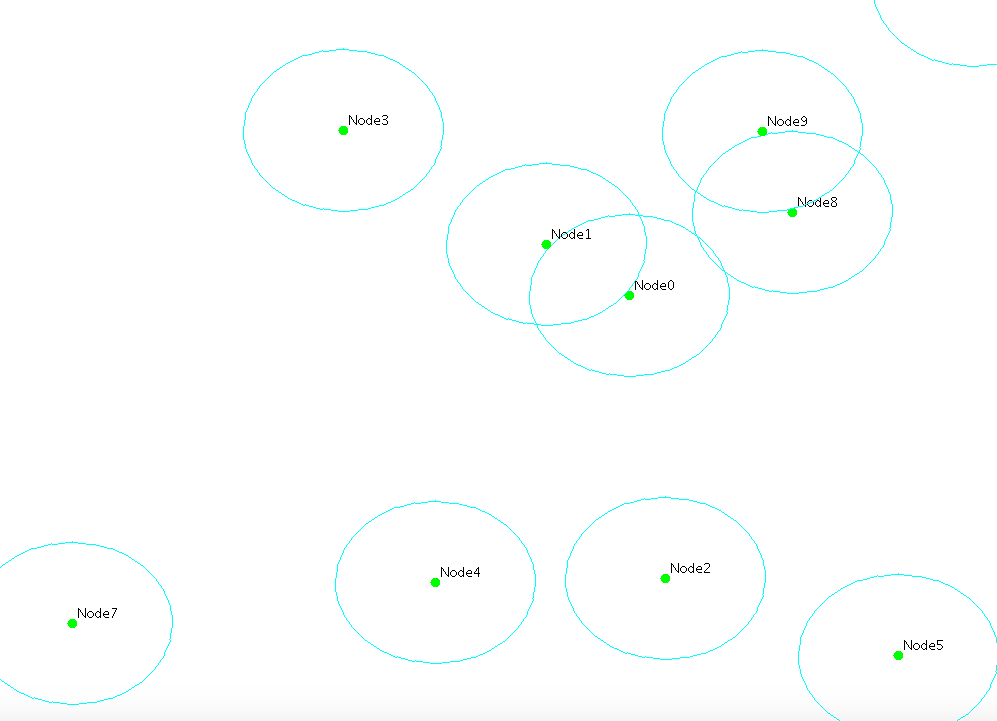
\includegraphics[height = 0.2\textheight,width = 1\textwidth]{imgs/1.png}
 		\caption[cap1]{Capture 1}
        \label{fig:Capture 1}
\end{flushleft}\end{minipage}
\begin{minipage}{0.4\textwidth} \begin{flushright}
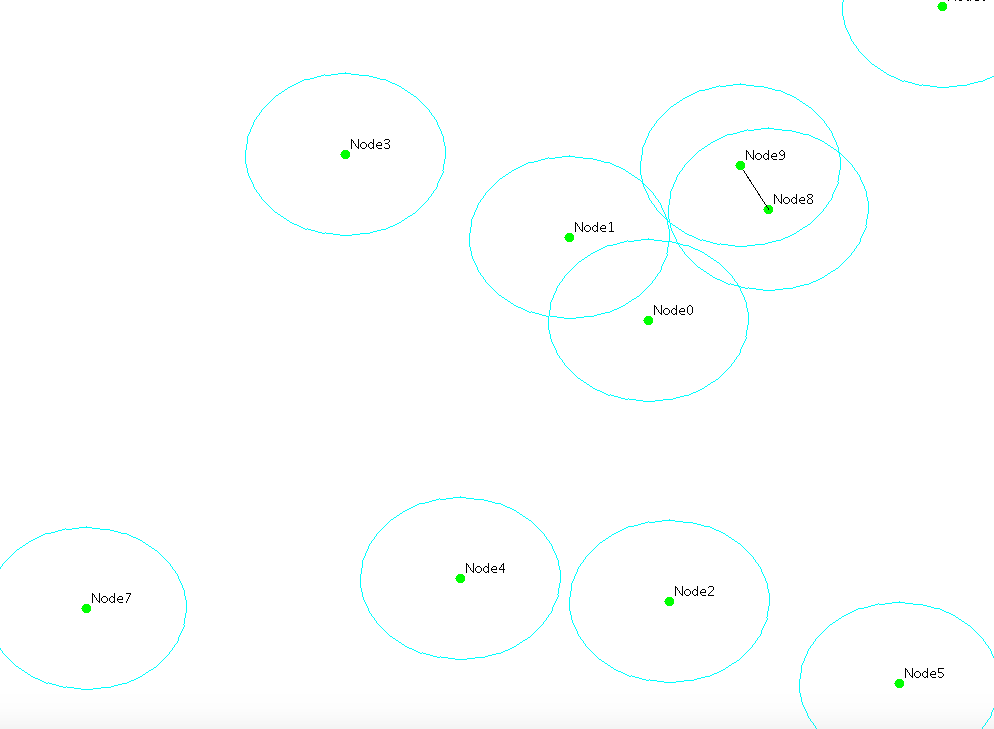
\includegraphics[height = 0.2\textheight,width = 1\textwidth]{imgs/2.png}
 		\caption[cap2]{Capture 2}
        \label{fig:Capture 2}
\end{flushright}\end{minipage}
\begin{minipage}{0.4\textwidth} \begin{flushleft}
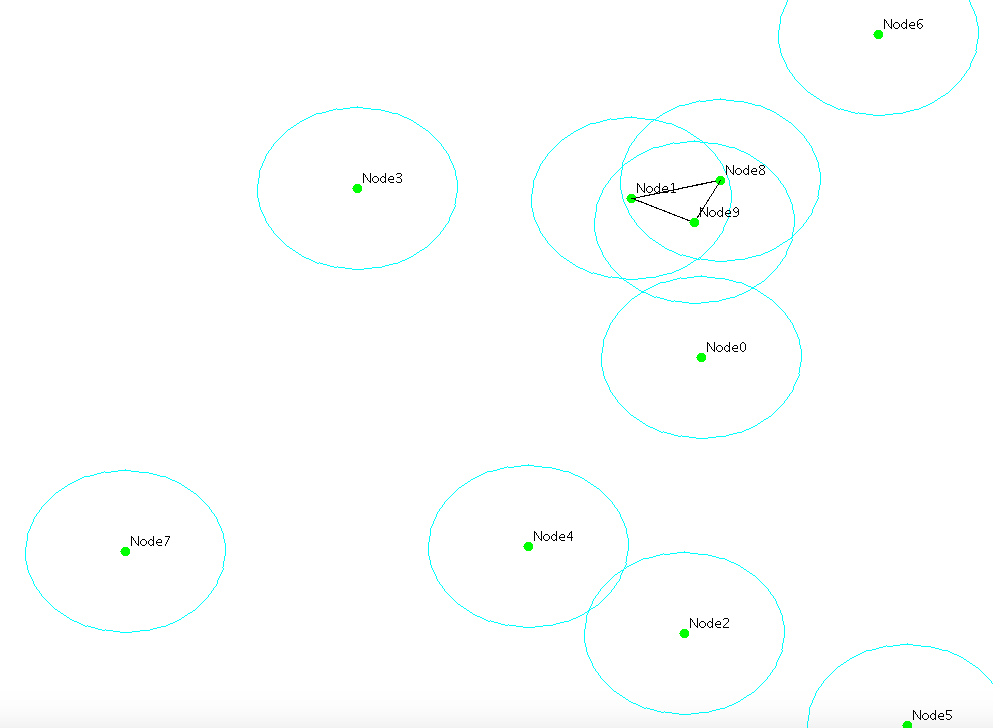
\includegraphics[height = 0.2\textheight,width = 1\textwidth]{imgs/3.png}
 		\caption[cap1]{Capture 3}
        \label{fig:Capture 3}
\end{flushleft}\end{minipage}
\begin{minipage}{0.4\textwidth} \begin{flushright}
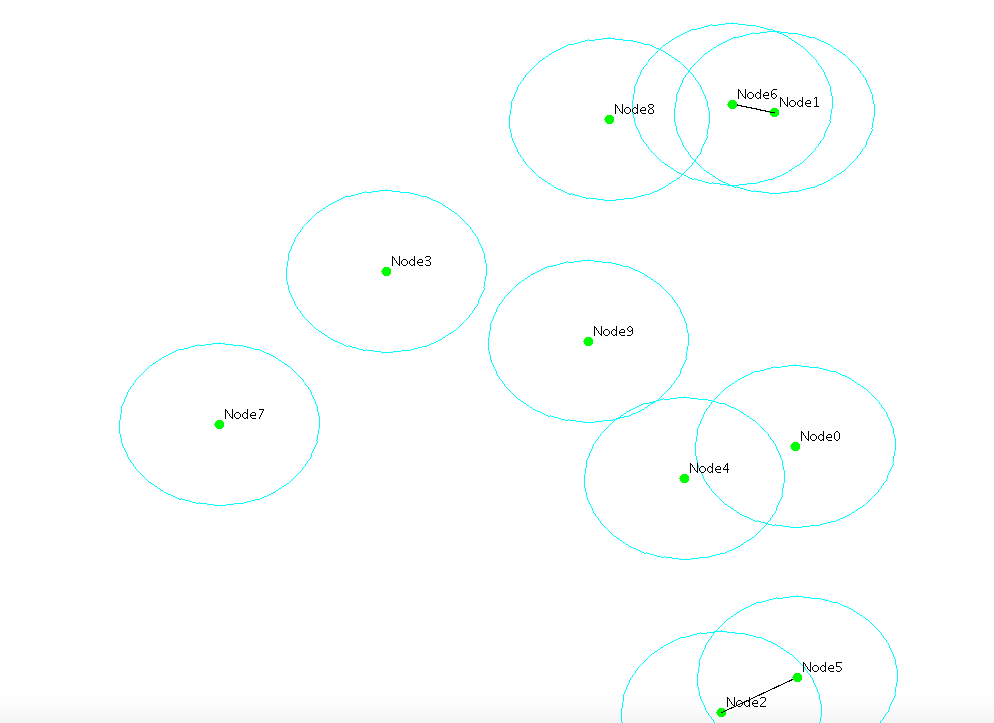
\includegraphics[height = 0.2\textheight,width = 1\textwidth]{imgs/4.png}
 		\caption[cap2]{Capture 4}
        \label{fig:Capture 4}
\end{flushright}\end{minipage}
\end{center}
\end{figure}

\subsection{Question 8}

Le tableau ci-dessous montre la connexité à termes des combinaisons des différentes stratégies dans les mêmes conditions de simulation que celles des questions précédentes (10 nœuds et une fenêtre de 1000 x 1000).({\color{red}si nous faisons baisser le nombre de nœuds à 2 par exemple, certaines des affirmations du tableau ne seront plus vraies} ou {\color{green}si nous changeons la valeur du scope à 300})\\

\begin{center}
\begin{tabular}{|l|l|l|l|l|}
  \hline
  SD/SPI & Strategy1InitNext & Strategy3InitNext & Strategy5Init & Strategy6Init \\
  \hline
	Strategy1InitNext & Non 			& Non 			 & Non & Non \\
  \hline
	Strategy2Next     & Non 			& \color{red}Oui & Oui & Oui \\
  \hline
	Strategy3InitNext & \color{red}Oui  & \color{red}Oui & Non & \color{red}Oui \\
  \hline
	Strategy4Next     & \color{green}Non 			& Oui 			 & Oui & Oui \\
  \hline
\end{tabular}
\captionof{table}{Combinaisons SD/SPI et connexité à termes}
\end{center}

La stratégie \textbf{(Strategy3InitNext)} réduit la fenêtre à un carré centré au milieu et de coté égal à 2 x (scope - marge) où marge est le minimum entre scope et 20.\\

La stratégie \textbf{(Strategy4Next)} génère une nouvelle position du noeud en fonction des voisins aux quels il est connecté en choisissant un angle et une distance dans [0, scope] en faisant bouger un nœud à la fois.\\

La stratégie \textbf{(Strategy5Init)} réduit la fenêtre au moment de l'initialisation des positions à un rectangle entre [maxX/3,maxY/3] et [maxX,maxY] ou une position en fonction de celle de l'un des voisins sur toute la fenêtre.\\

La stratégie \textbf{(Strategy6Init)} positionne les nœuds du réseau sous forme d'une étoile centrée au milieu de la fenêtre avec deux niveaux de nœuds (d'id pairs et impairs) éloignés d'une distance de scope/2.\\

\subsection{Question 9}

\noindent\begin{minipage}{\textwidth}
\begin{shaded}
\begin{boxedlisting}
public class DensityController implements Control{

	private static final String PAR_NEIGHBORPID = "neighborprotocol";

	private int neighbour_pid;
	private NeighborProtocolImpl neighbourProt;
	private List<Double> densities;
	private List<Double> standardDeviations;
	
	public DensityController(String prefix) {
		neighbour_pid = Configuration.getPid(prefix+"."+PAR_NEIGHBORPID);
		densities = new ArrayList<Double>();
		standardDeviations  = new ArrayList<Double>();
	}

	@Override
	public boolean execute() {
		densities.add(getDensity());
		standardDeviations.add(getStandardDeviation());
		return false;
	}

	public double getDensity() {
		double sum = 0;
		for(int i = 0;i < Network.size();i++) {
			neighbourProt = (NeighborProtocolImpl)Network.get(i).getProtocol(neighbour_pid);
			sum += neighbourProt.getNeighbors().size();
		}
		return sum/Network.size();
	}
	
	public double getStandardDeviation() {
		double density = getDensity();
		double sum = 0;
		for (int i = 0; i<Network.size(); i++) {
			neighbourProt = (NeighborProtocolImpl)Network.get(i).getProtocol(neighbour_pid);
			 sum += Math.pow(((double)neighbourProt.getNeighbors().size() - density),2) ;
		}
		return Math.sqrt(sum/Network.size());
	}
	
	public double getAverageDensity() {
		double sum = 0;
		for (int i = 0; i < densities.size(); i++) {
			sum += densities.get(i);
		}
		return sum/densities.size();
	}
	
	public double getAverageStandardDeviation() {
		double sum = 0;
		for (int i =0; i< standardDeviations.size(); i++) {
			sum += standardDeviations.get(i);
		}
		return sum/standardDeviations.size();
	}
	
	public double getDensityStandardDeviation() {
		double sum = 0;
		double num = getAverageDensity();
		for (int i = 0; i < densities.size(); i++) {
			sum += Math.pow((densities.get(i) - num),2);
		}
		return Math.sqrt(sum/densities.size());
	}	
}
\end{boxedlisting}
\end{shaded}
\end{minipage}

\subsection{Question 10}
Le tableau complété :\\

\begin{center}
\begin{tabular}{|l|l|l|l|l|l|}
  \hline
  Portée & SPI & SD & D($t_{end}$) & $\frac{E(t_{end})}{D(t_{end})}$ & $\frac{ED(t_{end})}{D(t_{end})}$\\
  \hline
	125 & 1 & 1 & 0 & 0 & 0\\
  \hline
	250 & 1 & 1 & 0 & 0 & 0\\
  \hline
	375 & 1 & 1 & 0 & 0 & 0\\
  \hline
	500 & 1 & 1 & 0 & 0 & 0\\
  \hline
	625 & 1 & 1 & 0 & 0 & 0\\
  \hline
	750 & 1 & 1 & 0 & 0 & 0\\
  \hline
	875 & 1 & 1 & 0 & 0 & 0\\
  \hline
	1000 & 1 & 1 & 0 & 0 & 0\\
  \hline
	125 & 3 & 3 & 0 & 0 & 0\\
  \hline
	250 & 3 & 3 & 0 & 0 & 0\\
  \hline
	375 & 3 & 3 & 0 & 0 & 0\\
  \hline
	500 & 3 & 3 & 0 & 0 & 0\\
  \hline
	625 & 3 & 3 & 0 & 0 & 0\\
  \hline
	750 & 3 & 3 & 0 & 0 & 0\\
  \hline
	875 & 3 & 3 & 0 & 0 & 0\\
  \hline
	1000 & 3 & 3 & 0 & 0 & 0\\
  \hline
\end{tabular}
\end{center}

\subsection{Question 11}

L'impact de la portée (scope) sur \textbf{(Strategy1InitNext)} :\\

L'impact de la portée (scope) sur \textbf{(Strategy3InitNext)} :\\

\newpage
\section{Exercice 2  Étude de protocoles de diffusion}
\subsection{Question 1}
Le tableau complété :\\

\begin{center}
\begin{tabular}{|l|l|l|}
  \hline
  Taille réseau & D($t_{end}$) & $\frac{ED(t_{end})}{D(t_{end})}$\\
  \hline
	20 & 0 & 0\\
  \hline
  	30 & 0 & 0\\
  \hline
  	40 & 0 & 0\\
  \hline
  	50 & 0 & 0\\
  \hline
  	60 & 0 & 0\\
  \hline
  	70 & 0 & 0\\
  \hline
        80 & 0 & 0\\
  \hline
  	90 & 0 & 0\\
  \hline
  	100 & 0 & 0\\
  \hline
  	120 & 0 & 0\\
  \hline
  	140 & 0 & 0\\
  \hline
  	160 & 0 & 0\\
  \hline
  	180 & 0 & 0\\
  \hline
  	200 & 0 & 0\\
  \hline
\end{tabular}
\end{center}

\subsection{Question 2}
\subsection{Question 3}
\subsection{Question 4}
\subsection{Question 5}
\subsection{Question 6}
\subsection{Question 7}
\subsection{Question 8}
\subsection{Question 9}
%-------------------------------------------------------------------------------
% REFERENCES
%-------------------------------------------------------------------------------
\newpage
\section*{Références}
\href{https://pages.lip6.fr/Jonathan.Lejeune/}{Jonathan Lejeune}, Devoir ARA, \textit{MANET.} \href{https://pages.lip6.fr/Jonathan.Lejeune/documents/enseignements/ARA/sujet\_devoir\_2017\_2018.pdf}{Énoncé}, Décembre 2017.
\newline
\newline
\end{document}
%-------------------------------------------------------------------------------
% SNIPPETS
%-------------------------------------------------------------------------------

%\begin{figure}[!ht]
%	\centering
%	\includegraphics[width=0.8\textwidth]{file_name}
%	\caption{}
%	\centering
%	\label{label:file_name}
%\end{figure}

%\begin{figure}[!ht]
%	\centering
%	\includegraphics[width=0.8\textwidth]{graph}
%	\caption{Blood pressure ranges and associated level of hypertension (American Heart Association, 2013).}
%	\centering
%	\label{label:graph}
%\end{figure}

%\begin{wrapfigure}{r}{0.30\textwidth}
%	\vspace{-40pt}
%	\begin{center}
%		\includegraphics[width=0.29\textwidth]{file_name}
%	\end{center}
%	\vspace{-20pt}
%	\caption{}
%	\label{label:file_name}
%\end{wrapfigure}

%\begin{wrapfigure}{r}{0.45\textwidth}
%	\begin{center}
%		\includegraphics[width=0.29\textwidth]{manometer}
%	\end{center}
%	\caption{Aneroid sphygmomanometer with stethoscope (Medicalexpo, 2012).}
%	\label{label:manometer}
%\end{wrapfigure}

%\begin{table}[!ht]\footnotesize
%	\centering
%	\begin{tabular}{cccccc}
%	\toprule
%	\multicolumn{2}{c} {Pearson's correlation test} & \multicolumn{4}{c} {Independent t-test} \\
%	\midrule	
%	\multicolumn{2}{c} {Gender} & \multicolumn{2}{c} {Activity level} & \multicolumn{2}{c} {Gender} \\
%	\midrule
%	Males & Females & 1st level & 6th level & Males & Females \\
%	\midrule
%	\multicolumn{2}{c} {BMI vs. SP} & \multicolumn{2}{c} {Systolic pressure} & \multicolumn{2}{c} {Systolic Pressure} \\
%	\multicolumn{2}{c} {BMI vs. DP} & \multicolumn{2}{c} {Diastolic pressure} & \multicolumn{2}{c} {Diastolic pressure} \\
%	\multicolumn{2}{c} {BMI vs. MAP} & \multicolumn{2}{c} {MAP} & \multicolumn{2}{c} {MAP} \\
%	\multicolumn{2}{c} {W:H ratio vs. SP} & \multicolumn{2}{c} {BMI} & \multicolumn{2}{c} {BMI} \\
%	\multicolumn{2}{c} {W:H ratio vs. DP} & \multicolumn{2}{c} {W:H ratio} & \multicolumn{2}{c} {W:H ratio} \\
%	\multicolumn{2}{c} {W:H ratio vs. MAP} & \multicolumn{2}{c} {\% Body fat} & \multicolumn{2}{c} {\% Body fat} \\
%	\multicolumn{2}{c} {} & \multicolumn{2}{c} {Height} & \multicolumn{2}{c} {Height} \\
%	\multicolumn{2}{c} {} & \multicolumn{2}{c} {Weight} & \multicolumn{2}{c} {Weight} \\
%	\multicolumn{2}{c} {} & \multicolumn{2}{c} {Heart rate} & \multicolumn{2}{c} {Heart rate} \\
%	\bottomrule
%	\end{tabular}
%	\caption{Parameters that were analysed and related statistical test performed for current study. BMI - body mass index; SP - systolic pressure; DP - diastolic pressure; MAP - mean arterial pressure; W:H ratio - waist to hip ratio.}
%	\label{label:tests}
%\end{table}\documentclass[10pt]{report}

%%%%%%%%%%%%%%%%%%%%%%%%%%%%%%%%%% DEBUT DU PREAMBULE %%%%%%%%%%%%%%%%%%%%%%%%%%%%%%%%%
\title{Rapport Devoir ARA}															%%%
\usepackage[francais]{babel}														%%%
\usepackage[T1]{fontenc}															%%%
\usepackage[utf8]{inputenc}															%%%
\usepackage{fancyhdr}																%%%
\usepackage{lastpage}																%%%
\usepackage{graphicx, wrapfig, subcaption, setspace, booktabs}						%%%
\usepackage[T1]{fontenc}															%%%
\usepackage[font=small, labelfont=bf]{caption}										%%%
\usepackage{fourier}																%%%
\usepackage[protrusion=true, expansion=true]{microtype}								%%%
\usepackage{sectsty}																%%%
\usepackage{url}																	%%%
\usepackage[colorlinks=true, urlcolor=blue, linkcolor=black]{hyperref}				%%%
\usepackage[margin=1in]{geometry}													%%%
\renewcommand\thesection{\arabic{section}}											%%%
\newcommand{\HRule}[1]{\rule{\linewidth}{#1}}										%%%
\onehalfspacing																		%%%
\setcounter{tocdepth}{5}															%%%
\setcounter{secnumdepth}{5}															%%%
\usepackage[]{array}                                                                %%%
\usepackage{mathtools}																%%%
\usepackage{underscore}
%%%%%%%%%%%%%%%%%%%%%%%%%%%%%%%%%% FIN DU PREAMBULE %%%%%%%%%%%%%%%%%%%%%%%%%%%%%%%%%%%

%--------
\usepackage[pdftex]{xcolor}
\usepackage{tcolorbox,listings}
\usepackage{framed}
\usepackage{tcolorbox}

\newenvironment{roundedframe}{%
  \def\FrameCommand{\tcbox[arc=5mm,colframe=red]}%
  \MakeFramed {\advance\hsize-\width \FrameRestore}}%
 {\endMakeFramed}

\definecolor{javared}{rgb}{0.6,0,0} % for strings
\definecolor{javagreen}{rgb}{0.25,0.5,0.35} % comments
\definecolor{javapurple}{rgb}{0.5,0,0.35} % keywords
\definecolor{javadocblue}{rgb}{0.25,0.35,0.75} % javadoc
\definecolor{shadecolor}{rgb}{.94,.97,1}
\lstnewenvironment{boxedlisting}{
\lstset{language=Java,
basicstyle=\ttfamily,
keywordstyle=\color{javapurple}\bfseries,
stringstyle=\color{javared},
commentstyle=\color{javagreen},
morecomment=[s][\color{javadocblue}]{/**}{*/},
numbers=left,
numberstyle=\color{black},
stepnumber=1,
numbersep=8pt,
tabsize=2,
showspaces=false,
showstringspaces=false,
columns=fullflexible,
frame = single,
breaklines=true,
escapeinside={(*@}{@*)},
postbreak=\mbox{\textcolor{red}{$\hookrightarrow$}\space}
}}{}

\usepackage{etoolbox}
%\BeforeBeginEnvironment{boxedlisting}{\begin{roundedframe}}
%\AfterEndEnvironment{boxedlisting}{\end{roundedframe}}

%--------


%-------------------------------------------------------------------------------
% HEADER & FOOTER
%-------------------------------------------------------------------------------
\pagestyle{fancy}
\fancyhf{}
\setlength\headheight{15pt}
\fancyhead[L]{BENTAHAR \& AINAS}
\fancyhead[R]{UPMC}
\fancyfoot[R]{Page \thepage\ / \pageref{LastPage}}
%-------------------------------------------------------------------------------
% TITLE PAGE
%-------------------------------------------------------------------------------

\begin{document}

\title{ \normalsize \textsc{\LARGE {Systèmes et Applications Répartis}\\\Large{Algorithmique Répartie Avancée}}
		\\ [2.0cm]
		\HRule{0.5pt} \\
		\LARGE \textbf{\uppercase{Devoir ARA 2017-2018\\MANET}}
		\HRule{2pt} \\ [0.5cm]
		\normalsize \vspace*{3\baselineskip}}

\author{
		Athmane BENTAHAR (3410322)\\Tacfarinas AINAS (3001048)}

\maketitle
\tableofcontents
\newpage
%-------------------------------------------------------------------------------
% Section title formatting
%-------------------------------------------------------------------------------
\sectionfont{\scshape}
%-------------------------------------------------------------------------------
% BODY
%-------------------------------------------------------------------------------
\section{Introduction}
\section{Exercice 1  Implémentation d'un MANET dans PeerSim}
\subsection{Question 1}

Initialement, un objet de la classe doit avoir \\
-une vitesse (entre min et max) qu'il peut avoir quand il est en mouvement, \\
-un temps lorsqu'il est en pause, \\
-et avoir connaissance de la longueur et largeur de la frame dans laquelle les nœuds pourront agir. \\
Il doit aussi avoir des stratégies de positions qui vont permettre au noeuds de savoir, initialement et dans l'exécution, les positions qu'ils auront. \\
Déplacement du noeud : \\
1) Lorsque le noeud n'est pas en mouvement, c'est à dire initialement où lorsqu'il est en pause, on calcule une vitesse alétoire entre min et max, puis on calcule la position destination selon la vitesse calculée et la stratégie NextDestination adoptée. \\
2) Si on a pas atteint la destination, on avance vers elle en ligne droite jusqu'à l'atteindre, puis on se met en pause et on réitère 1) \\
\subsection{Question 2}
Voici le contenu du fichier de configuration à ce point du projet :
\newline
\newline
\noindent\begin{minipage}{\textwidth}
\begin{shaded}
\begin{boxedlisting}
random.seed 5
network.size 10
simulation.endtime 100000
################### protocols ===========================
protocol.pos manet.positioning.PositionProtocolImpl
protocol.pos.maxspeed 100
protocol.pos.minspeed 50
protocol.pos.width 1000
protocol.pos.height 1000
protocol.pos.pause 10
################### initialization ======================
# initializer
init.initial manet.positioning.Initialize
init.initial.positionprotocol pos
# strategies
initial_position_strategy manet.positioning.strategies.Strategy1InitNext
initial_position_strategy.positionprotocol pos
next_destination_strategy manet.positioning.strategies.Strategy1InitNext
next_destination_strategy.positionprotocol pos
################ control ==============================
control.graph manet.GraphicalMonitor
control.graph.positionprotocol pos
control.graph.step 2
control.graph.time_slow 0.0002
\end{boxedlisting}
\end{shaded}
\end{minipage}

\subsection{Question 3}
La stratégie \textbf{(Strategy1InitNext)} initialise les positions des nœuds du réseau dans l'espace compris entre [0,maxX] et [0,maxY], en générant une position (aléatoire) et une vitesse initiale nulle. Aussi fait mouvoir les nœuds à chaque appel en générant une nouvelle position (aléatoire).

\subsection{Question 4}
La stratégie \textbf{(Strategy2Next)} ne fait que restituer la position actuelle du nœud comme nouvelle position. Ce qui mène à une immobilité des nœuds.

\subsection{Question 5}

\noindent\begin{minipage}{\textwidth}
\begin{shaded}
\begin{boxedlisting}
@Override
public void emit(Node host, Message msg) {
	for (int i = 0; i < Network.getCapacity(); i++) { // For all network
															// nodes
		node = Network.get(i);
		if (host.getID() != node.getID()) { // Except me
			if (host.getID() == msg.getIdDest()) { // I am the recipient of
														// the received message
				hostPos = (PositionProtocol) host.getProtocol(position_pid);
				nodePos = (PositionProtocol) node.getProtocol(position_pid);
				if ((hostPos.getCurrentPosition().distance(nodePos.getCurrentPosition()) <= this.getScope())) {
					EDSimulator.add(this.getLatency(), msg, node, position_pid); // Send()
				}
			}
		}
	}
}
\end{boxedlisting}
\end{shaded}
\end{minipage}

\subsection{Question 6}

\noindent\begin{minipage}{\textwidth}
\begin{shaded}
\begin{boxedlisting}
public class NeighborProtocolImpl implements NeighborProtocol, EDProtocol {

	private static final String PAR_EMITTERPID = "emitterprotocol";
	private static final String PAR_PERIOD = "period";
	private static final String PAR_DELTA = "delta";

	private final int neighbour_pid;
	private final int emitter_pid;
	private final long period;
	private final long delta;
	private List<Long> neighbours;
	private List<Long> periodN;
	private Message msg;
	
	public NeighborProtocolImpl(String prefix) {
		String tmp[] = prefix.split("\\.");
		neighbour_pid = Configuration.lookupPid(tmp[tmp.length - 1]);
		emitter_pid = Configuration.getPid(prefix + "." + PAR_EMITTERPID);
		delta = Configuration.getInt(prefix + "." + PAR_DELTA);
		period = Configuration.getInt(prefix + "." + PAR_PERIOD);
	}

	@Override
	public List<Long> getNeighbors() {
		return this.neighbours;
	}

	public long getPeriod() {
		return this.period;
	}

	public long getDelta() {
		return this.delta;
	}

	public NeighborProtocolImpl clone() {
		try {
			neighbours = new ArrayList<Long>();
			periodN = new ArrayList<Long>();
			return (NeighborProtocolImpl) super.clone();
		} catch (Exception e) {
			System.out.println("Cloning NeighborProtocolImpl Failed !");
		}
		return null;
	}

	@Override
	public void processEvent(Node host, int pid, Object event) {
		if (neighbour_pid != pid) {
			throw new RuntimeException("Receive Event for wrong protocol");
		}
		if (event instanceof String) {
			msg = new Message(host.getID(), -1, "", MessageType.probe, neighbour_pid);
			switch ((String) event) {
			case MessageType.firstprobe:
				((EmitterImpl) host.getProtocol(emitter_pid)).emit(host, msg) ;
				EDSimulator.add(period, MessageType.probe, host, neighbour_pid);
				break;
			case MessageType.probe:
				((EmitterImpl) host.getProtocol(emitter_pid)).emit(host, msg);
				EDSimulator.add(period, MessageType.probe, host, neighbour_pid);
				break;
			case MessageType.timer:
				for (int i = 0; i < neighbours.size(); i++) {
					if (!periodN.contains(neighbours.get(i))) {
						neighbours.remove(i);
					}
				}
				periodN.clear();
				EDSimulator.add(delta, MessageType.timer, host, neighbour_pid);
				break;
			default:
				break;
			}
		} else if (event instanceof Message) {
			long id = ((Message) event).getIdSrc();
			if (!periodN.contains(id)) {
				periodN.add(id);
			}
			if (!neighbours.contains(id)) {
				neighbours.add(id);
			}
			
		} else {
			throw new RuntimeException("Received Event of unmatching type");
		}
	}
}
\end{boxedlisting}
\end{shaded}
\end{minipage}

\subsection{Question 7}

\begin{figure}[h]
\begin{center}
\begin{minipage}{0.4\textwidth} \begin{flushleft}
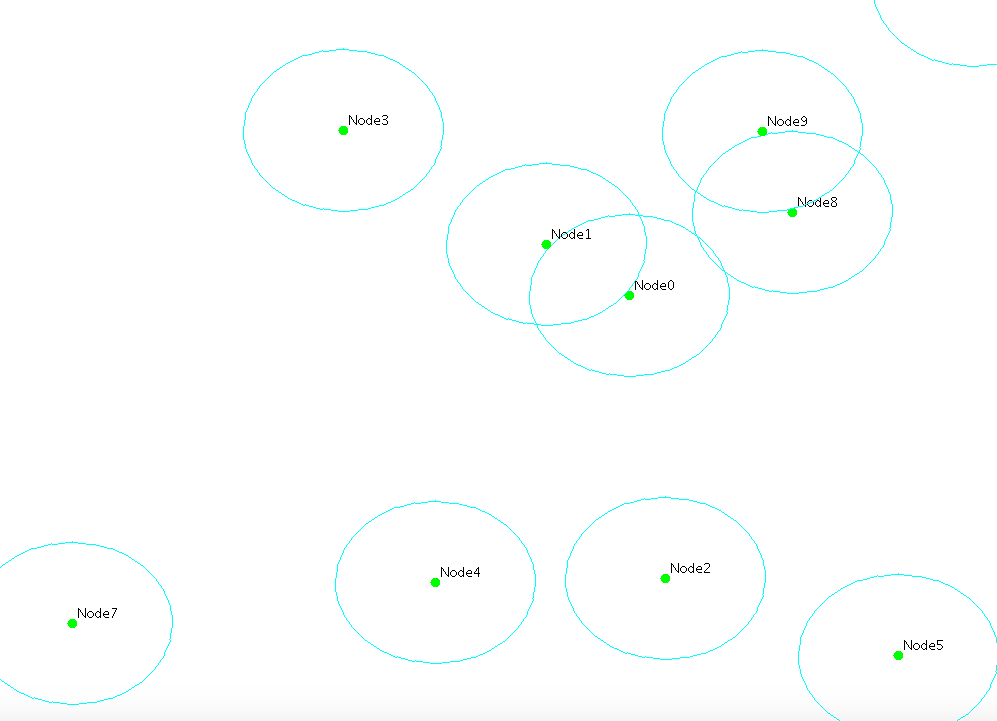
\includegraphics[height = 0.2\textheight,width = 1\textwidth]{imgs/1.png}
 		\caption[cap1]{Capture 1}
        \label{fig:Capture 1}
\end{flushleft}\end{minipage}
\begin{minipage}{0.4\textwidth} \begin{flushright}
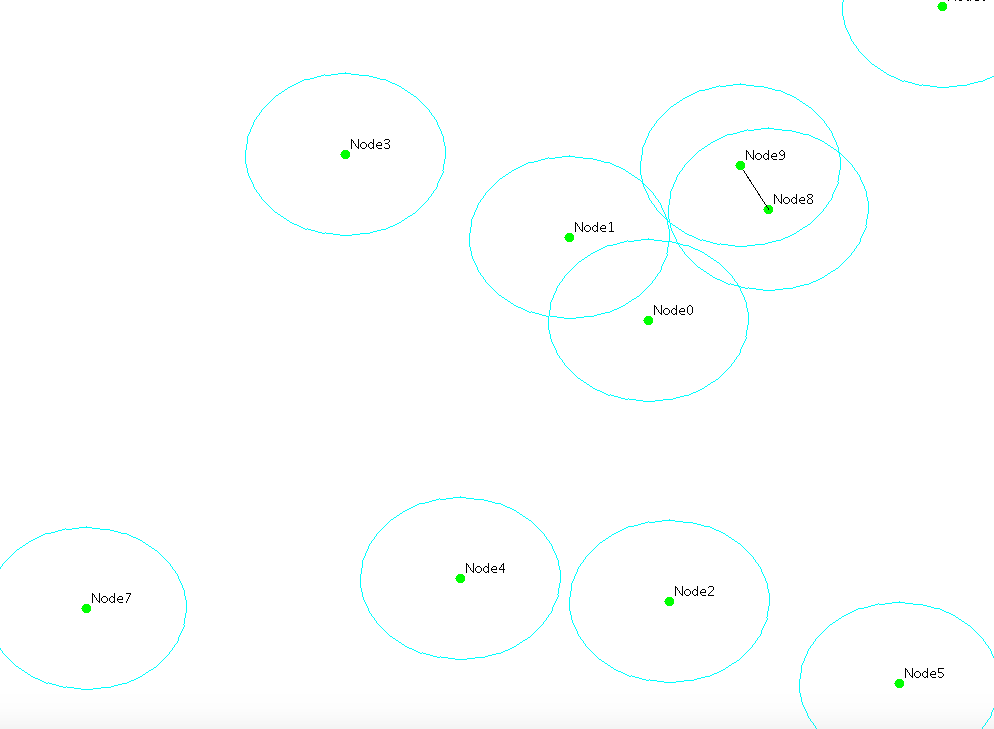
\includegraphics[height = 0.2\textheight,width = 1\textwidth]{imgs/2.png}
 		\caption[cap2]{Capture 2}
        \label{fig:Capture 2}
\end{flushright}\end{minipage}
\begin{minipage}{0.4\textwidth} \begin{flushleft}
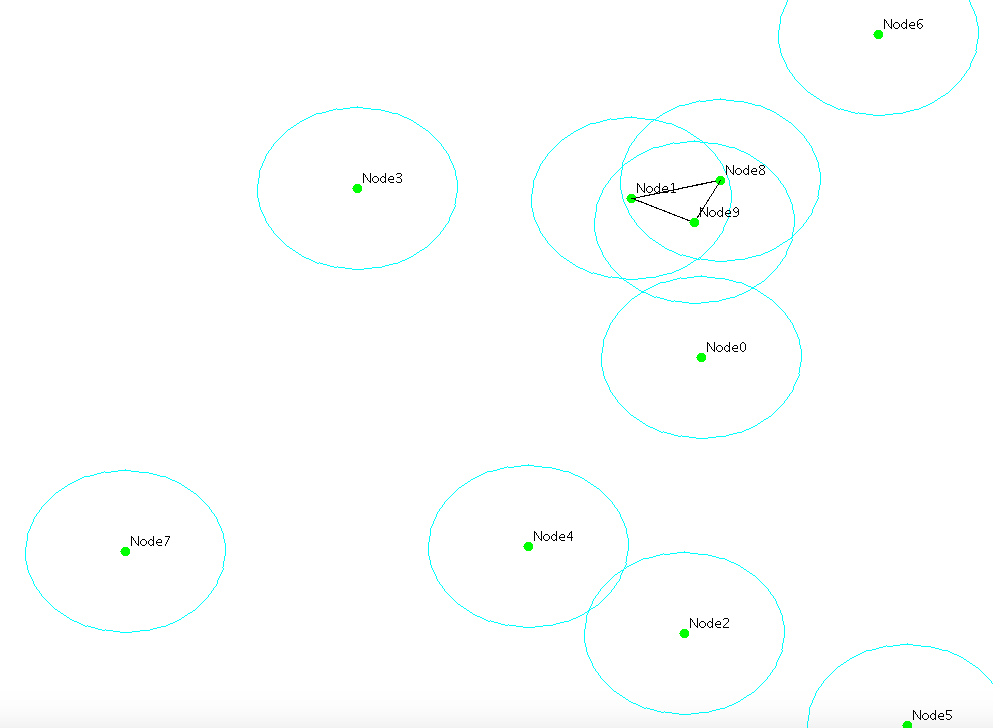
\includegraphics[height = 0.2\textheight,width = 1\textwidth]{imgs/3.png}
 		\caption[cap1]{Capture 3}
        \label{fig:Capture 3}
\end{flushleft}\end{minipage}
\begin{minipage}{0.4\textwidth} \begin{flushright}
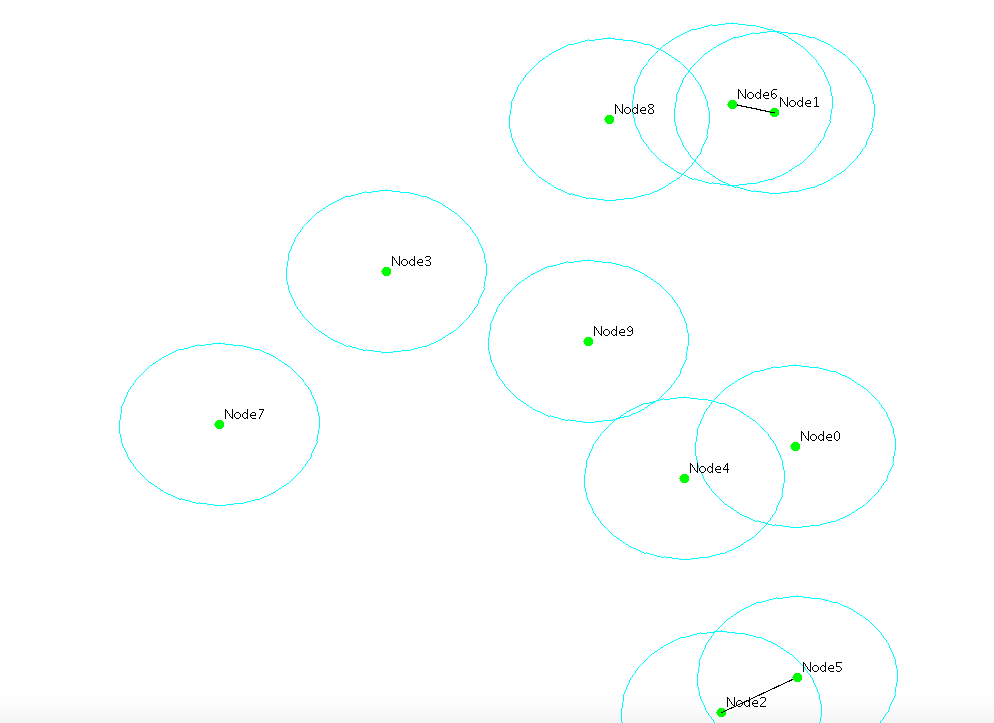
\includegraphics[height = 0.2\textheight,width = 1\textwidth]{imgs/4.png}
 		\caption[cap2]{Capture 4}
        \label{fig:Capture 4}
\end{flushright}\end{minipage}
\end{center}
\end{figure}

\subsection{Question 8}

Le tableau ci-dessous montre la connexité à termes des combinaisons des différentes stratégies dans les mêmes conditions de simulation que celles des questions précédentes (10 nœuds et une fenêtre de 1000 x 1000).({\color{red}si nous faisons baisser le nombre de nœuds à 2 par exemple, certaines des affirmations du tableau ne seront plus vraies} ou {\color{green}si nous changeons la valeur du scope à 300})\\

\begin{center}
\begin{tabular}{|l|l|l|l|l|}
  \hline
  SD/SPI & Strategy1InitNext & Strategy3InitNext & Strategy5Init & Strategy6Init \\
  \hline
	Strategy1InitNext & Non 			& Non 			 & Non & Non \\
  \hline
	Strategy2Next     & Non 			& \color{red}Oui & Oui & Oui \\
  \hline
	Strategy3InitNext & \color{red}Oui  & \color{red}Oui & Non & \color{red}Oui \\
  \hline
	Strategy4Next     & \color{green}Non 			& Oui 			 & Oui & Oui \\
  \hline
\end{tabular}
\captionof{table}{Combinaisons SD/SPI et connexité à termes}
\end{center}

La stratégie \textbf{(Strategy3InitNext)} réduit la fenêtre à un carré centré au milieu et de coté égal à 2 x (scope - marge) où marge est le minimum entre scope et 20.\\

La stratégie \textbf{(Strategy4Next)} génère une nouvelle position du noeud en fonction des voisins aux quels il est connecté en choisissant un angle et une distance dans [0, scope] en faisant bouger un nœud à la fois.\\

La stratégie \textbf{(Strategy5Init)} réduit la fenêtre au moment de l'initialisation des positions à un rectangle entre [maxX/3,maxY/3] et [maxX,maxY] ou une position en fonction de celle de l'un des voisins sur toute la fenêtre.\\

La stratégie \textbf{(Strategy6Init)} positionne les nœuds du réseau sous forme d'une étoile centrée au milieu de la fenêtre avec deux niveaux de nœuds (d'id pairs et impairs) éloignés d'une distance de scope/2.\\

\subsection{Question 9}

\noindent\begin{minipage}{\textwidth}
\begin{shaded}
\begin{boxedlisting}
public class DensityController implements Control{

	private static final String PAR_NEIGHBORPID = "neighborprotocol";

	private int neighbour_pid;
	private NeighborProtocolImpl neighbourProt;
	private List<Double> densities;
	private List<Double> standardDeviations;
	
	public DensityController(String prefix) {
		neighbour_pid = Configuration.getPid(prefix+"."+PAR_NEIGHBORPID);
		densities = new ArrayList<Double>();
		standardDeviations  = new ArrayList<Double>();
	}

	@Override
	public boolean execute() {
		densities.add(getDensity());
		standardDeviations.add(getStandardDeviation());
		return false;
	}

	public double getDensity() {
		double sum = 0;
		for(int i = 0;i < Network.size();i++) {
			neighbourProt = (NeighborProtocolImpl)Network.get(i).getProtocol(neighbour_pid);
			sum += neighbourProt.getNeighbors().size();
		}
		return sum/Network.size();
	}
	
	public double getStandardDeviation() {
		double density = getDensity();
		double sum = 0;
		for (int i = 0; i<Network.size(); i++) {
			neighbourProt = (NeighborProtocolImpl)Network.get(i).getProtocol(neighbour_pid);
			 sum += Math.pow(((double)neighbourProt.getNeighbors().size() - density),2) ;
		}
		return Math.sqrt(sum/Network.size());
	}
	
	public double getAverageDensity() {
		double sum = 0;
		for (int i = 0; i < densities.size(); i++) {
			sum += densities.get(i);
		}
		return sum/densities.size();
	}
	
	public double getAverageStandardDeviation() {
		double sum = 0;
		for (int i =0; i< standardDeviations.size(); i++) {
			sum += standardDeviations.get(i);
		}
		return sum/standardDeviations.size();
	}
	
	public double getDensityStandardDeviation() {
		double sum = 0;
		double num = getAverageDensity();
		for (int i = 0; i < densities.size(); i++) {
			sum += Math.pow((densities.get(i) - num),2);
		}
		return Math.sqrt(sum/densities.size());
	}	
}
\end{boxedlisting}
\end{shaded}
\end{minipage}

\subsection{Question 10}
Le tableau complété :\\

\begin{center}
\begin{tabular}{|l|l|l|l|l|l|}
  \hline
  Portée & SPI & SD & D($t_{end}$) & $\frac{E(t_{end})}{D(t_{end})}$ & $\frac{ED(t_{end})}{D(t_{end})}$\\
  \hline
	125 & 1 & 1 & 0 & 0 & 0\\
  \hline
	250 & 1 & 1 & 0 & 0 & 0\\
  \hline
	375 & 1 & 1 & 0 & 0 & 0\\
  \hline
	500 & 1 & 1 & 0 & 0 & 0\\
  \hline
	625 & 1 & 1 & 0 & 0 & 0\\
  \hline
	750 & 1 & 1 & 0 & 0 & 0\\
  \hline
	875 & 1 & 1 & 0 & 0 & 0\\
  \hline
	1000 & 1 & 1 & 0 & 0 & 0\\
  \hline
	125 & 3 & 3 & 0 & 0 & 0\\
  \hline
	250 & 3 & 3 & 0 & 0 & 0\\
  \hline
	375 & 3 & 3 & 0 & 0 & 0\\
  \hline
	500 & 3 & 3 & 0 & 0 & 0\\
  \hline
	625 & 3 & 3 & 0 & 0 & 0\\
  \hline
	750 & 3 & 3 & 0 & 0 & 0\\
  \hline
	875 & 3 & 3 & 0 & 0 & 0\\
  \hline
	1000 & 3 & 3 & 0 & 0 & 0\\
  \hline
\end{tabular}
\end{center}

\subsection{Question 11}

L'impact de la portée (scope) sur \textbf{(Strategy1InitNext)} :\\

L'impact de la portée (scope) sur \textbf{(Strategy3InitNext)} :\\

\newpage
\section{Exercice 2  Étude de protocoles de diffusion}
\subsection{Question 1}
Le tableau complété :\\

\begin{center}
\begin{tabular}{|l|l|l|}
  \hline
  Taille réseau & D($t_{end}$) & $\frac{ED(t_{end})}{D(t_{end})}$\\
  \hline
	20 & 0 & 0\\
  \hline
  	30 & 0 & 0\\
  \hline
  	40 & 0 & 0\\
  \hline
  	50 & 0 & 0\\
  \hline
  	60 & 0 & 0\\
  \hline
  	70 & 0 & 0\\
  \hline
        80 & 0 & 0\\
  \hline
  	90 & 0 & 0\\
  \hline
  	100 & 0 & 0\\
  \hline
  	120 & 0 & 0\\
  \hline
  	140 & 0 & 0\\
  \hline
  	160 & 0 & 0\\
  \hline
  	180 & 0 & 0\\
  \hline
  	200 & 0 & 0\\
  \hline
\end{tabular}
\end{center}

\subsection{Question 2}
\subsection{Question 3}
\subsection{Question 4}
\subsection{Question 5}
\subsection{Question 6}
\subsection{Question 7}
\subsection{Question 8}
\subsection{Question 9}
%-------------------------------------------------------------------------------
% REFERENCES
%-------------------------------------------------------------------------------
\newpage
\section*{Références}
\href{https://pages.lip6.fr/Jonathan.Lejeune/}{Jonathan Lejeune}, Devoir ARA, \textit{MANET.} \href{https://pages.lip6.fr/Jonathan.Lejeune/documents/enseignements/ARA/sujet\_devoir\_2017\_2018.pdf}{Énoncé}, Décembre 2017.
\newline
\newline
\end{document}
%-------------------------------------------------------------------------------
% SNIPPETS
%-------------------------------------------------------------------------------

%\begin{figure}[!ht]
%	\centering
%	\includegraphics[width=0.8\textwidth]{file_name}
%	\caption{}
%	\centering
%	\label{label:file_name}
%\end{figure}

%\begin{figure}[!ht]
%	\centering
%	\includegraphics[width=0.8\textwidth]{graph}
%	\caption{Blood pressure ranges and associated level of hypertension (American Heart Association, 2013).}
%	\centering
%	\label{label:graph}
%\end{figure}

%\begin{wrapfigure}{r}{0.30\textwidth}
%	\vspace{-40pt}
%	\begin{center}
%		\includegraphics[width=0.29\textwidth]{file_name}
%	\end{center}
%	\vspace{-20pt}
%	\caption{}
%	\label{label:file_name}
%\end{wrapfigure}

%\begin{wrapfigure}{r}{0.45\textwidth}
%	\begin{center}
%		\includegraphics[width=0.29\textwidth]{manometer}
%	\end{center}
%	\caption{Aneroid sphygmomanometer with stethoscope (Medicalexpo, 2012).}
%	\label{label:manometer}
%\end{wrapfigure}

%\begin{table}[!ht]\footnotesize
%	\centering
%	\begin{tabular}{cccccc}
%	\toprule
%	\multicolumn{2}{c} {Pearson's correlation test} & \multicolumn{4}{c} {Independent t-test} \\
%	\midrule	
%	\multicolumn{2}{c} {Gender} & \multicolumn{2}{c} {Activity level} & \multicolumn{2}{c} {Gender} \\
%	\midrule
%	Males & Females & 1st level & 6th level & Males & Females \\
%	\midrule
%	\multicolumn{2}{c} {BMI vs. SP} & \multicolumn{2}{c} {Systolic pressure} & \multicolumn{2}{c} {Systolic Pressure} \\
%	\multicolumn{2}{c} {BMI vs. DP} & \multicolumn{2}{c} {Diastolic pressure} & \multicolumn{2}{c} {Diastolic pressure} \\
%	\multicolumn{2}{c} {BMI vs. MAP} & \multicolumn{2}{c} {MAP} & \multicolumn{2}{c} {MAP} \\
%	\multicolumn{2}{c} {W:H ratio vs. SP} & \multicolumn{2}{c} {BMI} & \multicolumn{2}{c} {BMI} \\
%	\multicolumn{2}{c} {W:H ratio vs. DP} & \multicolumn{2}{c} {W:H ratio} & \multicolumn{2}{c} {W:H ratio} \\
%	\multicolumn{2}{c} {W:H ratio vs. MAP} & \multicolumn{2}{c} {\% Body fat} & \multicolumn{2}{c} {\% Body fat} \\
%	\multicolumn{2}{c} {} & \multicolumn{2}{c} {Height} & \multicolumn{2}{c} {Height} \\
%	\multicolumn{2}{c} {} & \multicolumn{2}{c} {Weight} & \multicolumn{2}{c} {Weight} \\
%	\multicolumn{2}{c} {} & \multicolumn{2}{c} {Heart rate} & \multicolumn{2}{c} {Heart rate} \\
%	\bottomrule
%	\end{tabular}
%	\caption{Parameters that were analysed and related statistical test performed for current study. BMI - body mass index; SP - systolic pressure; DP - diastolic pressure; MAP - mean arterial pressure; W:H ratio - waist to hip ratio.}
%	\label{label:tests}
%\end{table}\documentclass[10pt]{report}

%%%%%%%%%%%%%%%%%%%%%%%%%%%%%%%%%% DEBUT DU PREAMBULE %%%%%%%%%%%%%%%%%%%%%%%%%%%%%%%%%
\title{Rapport Devoir ARA}															%%%
\usepackage[francais]{babel}														%%%
\usepackage[T1]{fontenc}															%%%
\usepackage[utf8]{inputenc}															%%%
\usepackage{fancyhdr}																%%%
\usepackage{lastpage}																%%%
\usepackage{graphicx, wrapfig, subcaption, setspace, booktabs}						%%%
\usepackage[T1]{fontenc}															%%%
\usepackage[font=small, labelfont=bf]{caption}										%%%
\usepackage{fourier}																%%%
\usepackage[protrusion=true, expansion=true]{microtype}								%%%
\usepackage{sectsty}																%%%
\usepackage{url}																	%%%
\usepackage[colorlinks=true, urlcolor=blue, linkcolor=black]{hyperref}				%%%
\usepackage[margin=1in]{geometry}													%%%
\renewcommand\thesection{\arabic{section}}											%%%
\newcommand{\HRule}[1]{\rule{\linewidth}{#1}}										%%%
\onehalfspacing																		%%%
\setcounter{tocdepth}{5}															%%%
\setcounter{secnumdepth}{5}															%%%
\usepackage[]{array}                                                                %%%
\usepackage{mathtools}																%%%
\usepackage{underscore}
%%%%%%%%%%%%%%%%%%%%%%%%%%%%%%%%%% FIN DU PREAMBULE %%%%%%%%%%%%%%%%%%%%%%%%%%%%%%%%%%%

%--------
\usepackage[pdftex]{xcolor}
\usepackage{tcolorbox,listings}
\usepackage{framed}
\usepackage{tcolorbox}

\newenvironment{roundedframe}{%
  \def\FrameCommand{\tcbox[arc=5mm,colframe=red]}%
  \MakeFramed {\advance\hsize-\width \FrameRestore}}%
 {\endMakeFramed}

\definecolor{javared}{rgb}{0.6,0,0} % for strings
\definecolor{javagreen}{rgb}{0.25,0.5,0.35} % comments
\definecolor{javapurple}{rgb}{0.5,0,0.35} % keywords
\definecolor{javadocblue}{rgb}{0.25,0.35,0.75} % javadoc
\definecolor{shadecolor}{rgb}{.94,.97,1}
\lstnewenvironment{boxedlisting}{
\lstset{language=Java,
basicstyle=\ttfamily,
keywordstyle=\color{javapurple}\bfseries,
stringstyle=\color{javared},
commentstyle=\color{javagreen},
morecomment=[s][\color{javadocblue}]{/**}{*/},
numbers=left,
numberstyle=\color{black},
stepnumber=1,
numbersep=8pt,
tabsize=2,
showspaces=false,
showstringspaces=false,
columns=fullflexible,
frame = single,
breaklines=true,
escapeinside={(*@}{@*)},
postbreak=\mbox{\textcolor{red}{$\hookrightarrow$}\space}
}}{}

\usepackage{etoolbox}
%\BeforeBeginEnvironment{boxedlisting}{\begin{roundedframe}}
%\AfterEndEnvironment{boxedlisting}{\end{roundedframe}}

%--------


%-------------------------------------------------------------------------------
% HEADER & FOOTER
%-------------------------------------------------------------------------------
\pagestyle{fancy}
\fancyhf{}
\setlength\headheight{15pt}
\fancyhead[L]{BENTAHAR \& AINAS}
\fancyhead[R]{UPMC}
\fancyfoot[R]{Page \thepage\ / \pageref{LastPage}}
%-------------------------------------------------------------------------------
% TITLE PAGE
%-------------------------------------------------------------------------------

\begin{document}

\title{ \normalsize \textsc{\LARGE {Systèmes et Applications Répartis}\\\Large{Algorithmique Répartie Avancée}}
		\\ [2.0cm]
		\HRule{0.5pt} \\
		\LARGE \textbf{\uppercase{Devoir ARA 2017-2018\\MANET}}
		\HRule{2pt} \\ [0.5cm]
		\normalsize \vspace*{3\baselineskip}}

\author{
		Athmane BENTAHAR (3410322)\\Tacfarinas AINAS (3001048)}

\maketitle
\tableofcontents
\newpage
%-------------------------------------------------------------------------------
% Section title formatting
%-------------------------------------------------------------------------------
\sectionfont{\scshape}
%-------------------------------------------------------------------------------
% BODY
%-------------------------------------------------------------------------------
\section{Introduction}
\section{Exercice 1  Implémentation d'un MANET dans PeerSim}
\subsection{Question 1}

Initialement, un objet de la classe doit avoir \\
-une vitesse (entre min et max) qu'il peut avoir quand il est en mouvement, \\
-un temps lorsqu'il est en pause, \\
-et avoir connaissance de la longueur et largeur de la frame dans laquelle les nœuds pourront agir. \\
Il doit aussi avoir des stratégies de positions qui vont permettre au noeuds de savoir, initialement et dans l'exécution, les positions qu'ils auront. \\
Déplacement du noeud : \\
1) Lorsque le noeud n'est pas en mouvement, c'est à dire initialement où lorsqu'il est en pause, on calcule une vitesse alétoire entre min et max, puis on calcule la position destination selon la vitesse calculée et la stratégie NextDestination adoptée. \\
2) Si on a pas atteint la destination, on avance vers elle en ligne droite jusqu'à l'atteindre, puis on se met en pause et on réitère 1) \\
\subsection{Question 2}
Voici le contenu du fichier de configuration à ce point du projet :
\newline
\newline
\noindent\begin{minipage}{\textwidth}
\begin{shaded}
\begin{boxedlisting}
random.seed 5
network.size 10
simulation.endtime 100000
################### protocols ===========================
protocol.pos manet.positioning.PositionProtocolImpl
protocol.pos.maxspeed 100
protocol.pos.minspeed 50
protocol.pos.width 1000
protocol.pos.height 1000
protocol.pos.pause 10
################### initialization ======================
# initializer
init.initial manet.positioning.Initialize
init.initial.positionprotocol pos
# strategies
initial_position_strategy manet.positioning.strategies.Strategy1InitNext
initial_position_strategy.positionprotocol pos
next_destination_strategy manet.positioning.strategies.Strategy1InitNext
next_destination_strategy.positionprotocol pos
################ control ==============================
control.graph manet.GraphicalMonitor
control.graph.positionprotocol pos
control.graph.step 2
control.graph.time_slow 0.0002
\end{boxedlisting}
\end{shaded}
\end{minipage}

\subsection{Question 3}
La stratégie \textbf{(Strategy1InitNext)} initialise les positions des nœuds du réseau dans l'espace compris entre [0,maxX] et [0,maxY], en générant une position (aléatoire) et une vitesse initiale nulle. Aussi fait mouvoir les nœuds à chaque appel en générant une nouvelle position (aléatoire).

\subsection{Question 4}
La stratégie \textbf{(Strategy2Next)} ne fait que restituer la position actuelle du nœud comme nouvelle position. Ce qui mène à une immobilité des nœuds.

\subsection{Question 5}

\noindent\begin{minipage}{\textwidth}
\begin{shaded}
\begin{boxedlisting}
@Override
public void emit(Node host, Message msg) {
	for (int i = 0; i < Network.getCapacity(); i++) { // For all network
															// nodes
		node = Network.get(i);
		if (host.getID() != node.getID()) { // Except me
			if (host.getID() == msg.getIdDest()) { // I am the recipient of
														// the received message
				hostPos = (PositionProtocol) host.getProtocol(position_pid);
				nodePos = (PositionProtocol) node.getProtocol(position_pid);
				if ((hostPos.getCurrentPosition().distance(nodePos.getCurrentPosition()) <= this.getScope())) {
					EDSimulator.add(this.getLatency(), msg, node, position_pid); // Send()
				}
			}
		}
	}
}
\end{boxedlisting}
\end{shaded}
\end{minipage}



\subsection{Question 6}

\noindent\begin{minipage}{\textwidth}
\begin{shaded}
\begin{boxedlisting}
public class NeighborProtocolImpl implements NeighborProtocol, EDProtocol {

	private static final String PAR_EMITTERPID = "emitterprotocol";
	private static final String PAR_PERIOD = "period";
	private static final String PAR_DELTA = "delta";

	private final int neighbour_pid;
	private final int emitter_pid;
	private final long period;
	private final long delta;
	private List<Long> neighbours;
	private List<Long> periodN;
	private Message msg;
	
	public NeighborProtocolImpl(String prefix) {
		String tmp[] = prefix.split("\\.");
		neighbour_pid = Configuration.lookupPid(tmp[tmp.length - 1]);
		emitter_pid = Configuration.getPid(prefix + "." + PAR_EMITTERPID);
		delta = Configuration.getInt(prefix + "." + PAR_DELTA);
		period = Configuration.getInt(prefix + "." + PAR_PERIOD);
	}

	@Override
	public List<Long> getNeighbors() {
		return this.neighbours;
	}

	public long getPeriod() {
		return this.period;
	}

	public long getDelta() {
		return this.delta;
	}

	public NeighborProtocolImpl clone() {
		try {
			neighbours = new ArrayList<Long>();
			periodN = new ArrayList<Long>();
			return (NeighborProtocolImpl) super.clone();
		} catch (Exception e) {
			System.out.println("Cloning NeighborProtocolImpl Failed !");
		}
		return null;
	}

	@Override
	public void processEvent(Node host, int pid, Object event) {
		if (neighbour_pid != pid) {
			throw new RuntimeException("Receive Event for wrong protocol");
		}
		if (event instanceof String) {
			msg = new Message(host.getID(), -1, "", MessageType.probe, neighbour_pid);
			switch ((String) event) {
			case MessageType.firstprobe:
				((EmitterImpl) host.getProtocol(emitter_pid)).emit(host, msg) ;
				EDSimulator.add(period, MessageType.probe, host, neighbour_pid);
				break;
			case MessageType.probe:
				((EmitterImpl) host.getProtocol(emitter_pid)).emit(host, msg);
				EDSimulator.add(period, MessageType.probe, host, neighbour_pid);
				break;
			case MessageType.timer:
				for (int i = 0; i < neighbours.size(); i++) {
					if (!periodN.contains(neighbours.get(i))) {
						neighbours.remove(i);
					}
				}
				periodN.clear();
				EDSimulator.add(delta, MessageType.timer, host, neighbour_pid);
				break;
			default:
				break;
			}
		} else if (event instanceof Message) {
			long id = ((Message) event).getIdSrc();
			if (!periodN.contains(id)) {
				periodN.add(id);
			}
			if (!neighbours.contains(id)) {
				neighbours.add(id);
			}
			
		} else {
			throw new RuntimeException("Received Event of unmatching type");
		}
	}
}
\end{boxedlisting}
\end{shaded}
\end{minipage}

\subsection{Question 7}

\begin{figure}[h]
\begin{center}
\begin{minipage}{0.4\textwidth} \begin{flushleft}
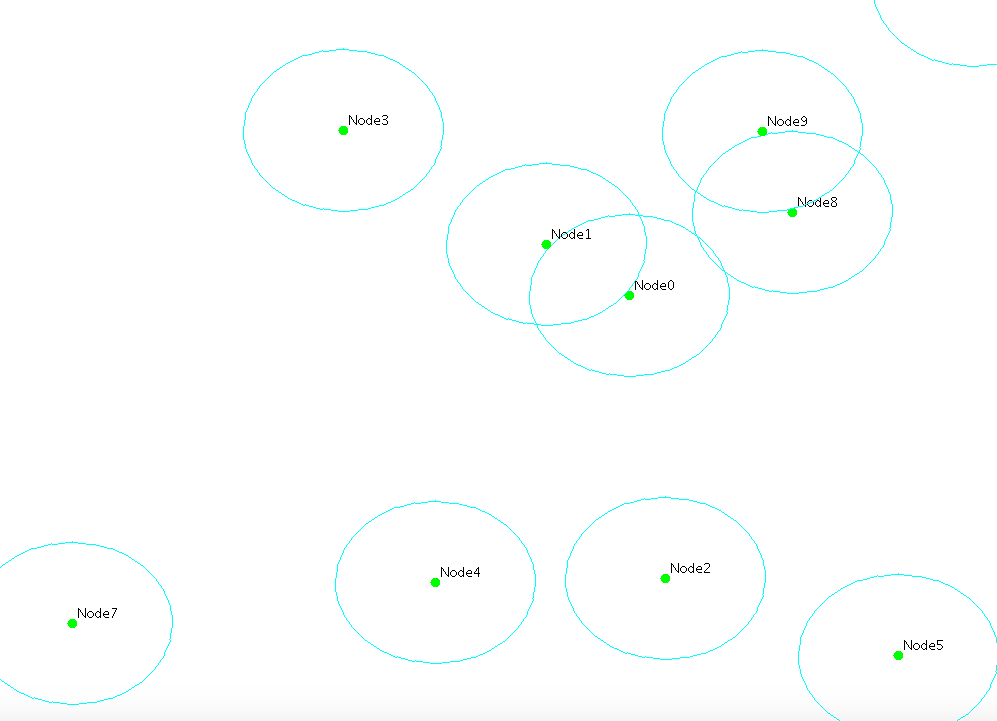
\includegraphics[height = 0.2\textheight,width = 1\textwidth]{imgs/1.png}
 		\caption[cap1]{Capture 1}
        \label{fig:Capture 1}
\end{flushleft}\end{minipage}
\begin{minipage}{0.4\textwidth} \begin{flushright}
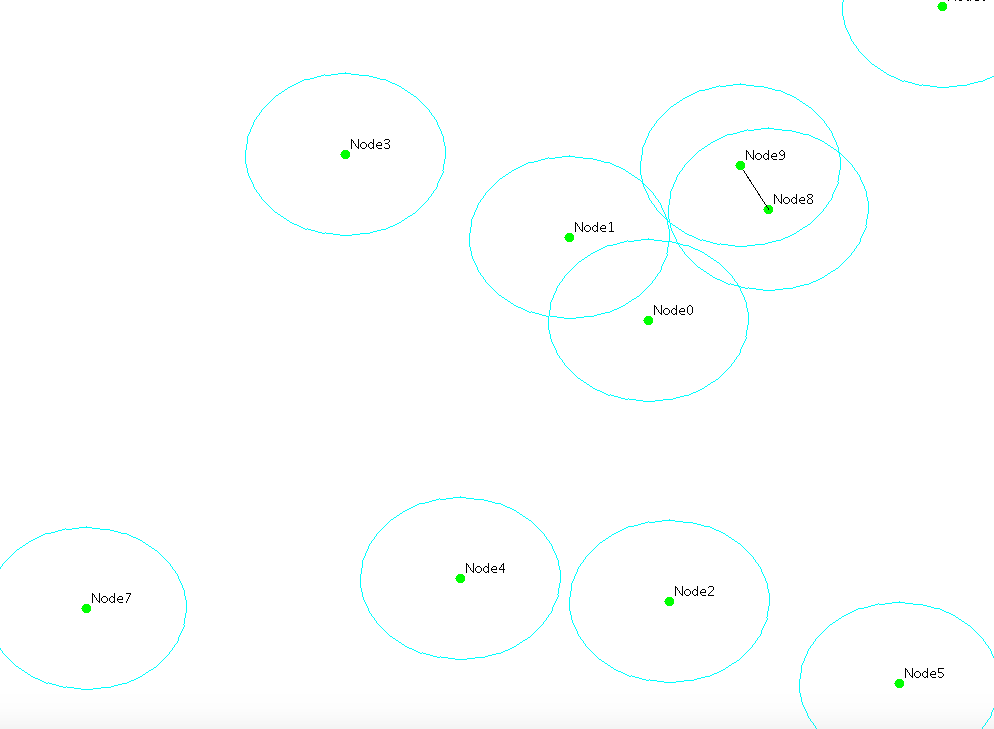
\includegraphics[height = 0.2\textheight,width = 1\textwidth]{imgs/2.png}
 		\caption[cap2]{Capture 2}
        \label{fig:Capture 2}
\end{flushright}\end{minipage}
\begin{minipage}{0.4\textwidth} \begin{flushleft}
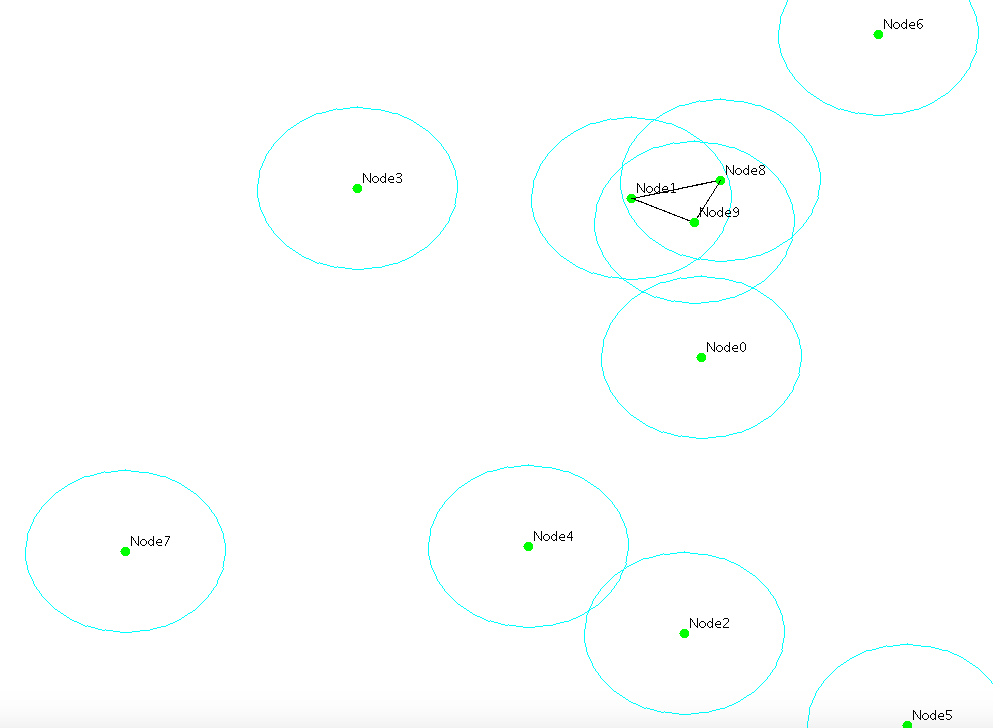
\includegraphics[height = 0.2\textheight,width = 1\textwidth]{imgs/3.png}
 		\caption[cap1]{Capture 3}
        \label{fig:Capture 3}
\end{flushleft}\end{minipage}
\begin{minipage}{0.4\textwidth} \begin{flushright}
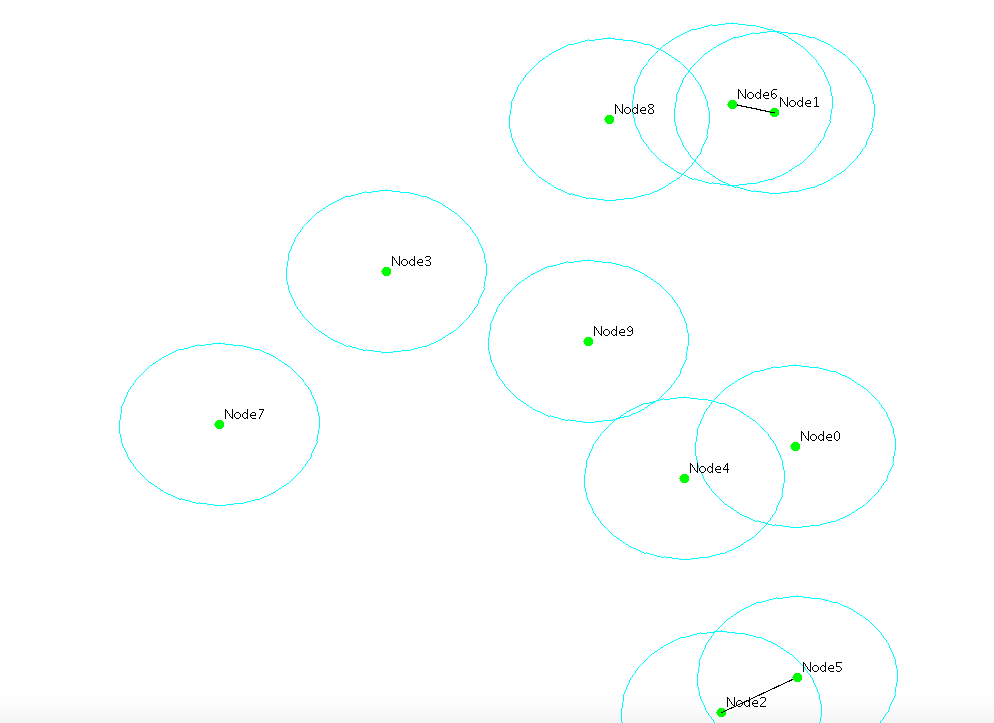
\includegraphics[height = 0.2\textheight,width = 1\textwidth]{imgs/4.png}
 		\caption[cap2]{Capture 4}
        \label{fig:Capture 4}
\end{flushright}\end{minipage}
\end{center}
\end{figure}

\subsection{Question 8}

Le tableau ci-dessous montre la connexité à termes des combinaisons des différentes stratégies dans les mêmes conditions de simulation que celles des questions précédentes (10 nœuds et une fenêtre de 1000 x 1000).({\color{red}si nous faisons baisser le nombre de nœuds à 2 par exemple, certaines des affirmations du tableau ne seront plus vraies} ou {\color{green}si nous changeons la valeur du scope à 300})\\

\begin{center}
\begin{tabular}{|l|l|l|l|l|}
  \hline
  SD/SPI & Strategy1InitNext & Strategy3InitNext & Strategy5Init & Strategy6Init \\
  \hline
	Strategy1InitNext & Non 			& Non 			 & Non & Non \\
  \hline
	Strategy2Next     & Non 			& \color{red}Oui & Oui & Oui \\
  \hline
	Strategy3InitNext & \color{red}Oui  & \color{red}Oui & Non & \color{red}Oui \\
  \hline
	Strategy4Next     & \color{green}Non 			& Oui 			 & Oui & Oui \\
  \hline
\end{tabular}
\captionof{table}{Combinaisons SD/SPI et connexité à termes}
\end{center}

La stratégie \textbf{(Strategy3InitNext)} réduit la fenêtre à un carré centré au milieu et de coté égal à 2 x (scope - marge) où marge est le minimum entre scope et 20.\\

La stratégie \textbf{(Strategy4Next)} génère une nouvelle position du noeud en fonction des voisins aux quels il est connecté en choisissant un angle et une distance dans [0, scope] en faisant bouger un nœud à la fois.\\

La stratégie \textbf{(Strategy5Init)} réduit la fenêtre au moment de l'initialisation des positions à un rectangle entre [maxX/3,maxY/3] et [maxX,maxY] ou une position en fonction de celle de l'un des voisins sur toute la fenêtre.\\

La stratégie \textbf{(Strategy6Init)} positionne les nœuds du réseau sous forme d'une étoile centrée au milieu de la fenêtre avec deux niveaux de nœuds (d'id pairs et impairs) éloignés d'une distance de scope/2.\\

\subsection{Question 9}
\subsection{Question 10}
Le tableau complété :\\

\begin{center}
\begin{tabular}{|l|l|l|l|l|l|}
  \hline
  Portée & SPI & SD & D($t_{end}$) & $\frac{E(t_{end})}{D(t_{end})}$ & $\frac{ED(t_{end})}{D(t_{end})}$\\
  \hline
	125 & 1 & 1 & 0 & 0 & 0\\
  \hline
	250 & 1 & 1 & 0 & 0 & 0\\
  \hline
	375 & 1 & 1 & 0 & 0 & 0\\
  \hline
	500 & 1 & 1 & 0 & 0 & 0\\
  \hline
	625 & 1 & 1 & 0 & 0 & 0\\
  \hline
	750 & 1 & 1 & 0 & 0 & 0\\
  \hline
	875 & 1 & 1 & 0 & 0 & 0\\
  \hline
	1000 & 1 & 1 & 0 & 0 & 0\\
  \hline
	125 & 3 & 3 & 0 & 0 & 0\\
  \hline
	250 & 3 & 3 & 0 & 0 & 0\\
  \hline
	375 & 3 & 3 & 0 & 0 & 0\\
  \hline
	500 & 3 & 3 & 0 & 0 & 0\\
  \hline
	625 & 3 & 3 & 0 & 0 & 0\\
  \hline
	750 & 3 & 3 & 0 & 0 & 0\\
  \hline
	875 & 3 & 3 & 0 & 0 & 0\\
  \hline
	1000 & 3 & 3 & 0 & 0 & 0\\
  \hline
\end{tabular}
\end{center}


\subsection{Question 11}
\newpage
\section{Exercice 2  Étude de protocoles de diffusion}
\subsection{Question 1}
Le tableau complété :\\

\begin{center}
\begin{tabular}{|l|l|l|}
  \hline
  Taille réseau & D($t_{end}$) & $\frac{ED(t_{end})}{D(t_{end})}$\\
  \hline
	20 & 0 & 0\\
  \hline
  	30 & 0 & 0\\
  \hline
  	40 & 0 & 0\\
  \hline
  	50 & 0 & 0\\
  \hline
  	60 & 0 & 0\\
  \hline
  	70 & 0 & 0\\
  \hline
        80 & 0 & 0\\
  \hline
  	90 & 0 & 0\\
  \hline
  	100 & 0 & 0\\
  \hline
  	120 & 0 & 0\\
  \hline
  	140 & 0 & 0\\
  \hline
  	160 & 0 & 0\\
  \hline
  	180 & 0 & 0\\
  \hline
  	200 & 0 & 0\\
  \hline
\end{tabular}
\end{center}

\subsection{Question 2}
\subsection{Question 3}
\subsection{Question 4}
\subsection{Question 5}
\subsection{Question 6}
\subsection{Question 7}
\subsection{Question 8}
\subsection{Question 9}
%-------------------------------------------------------------------------------
% REFERENCES
%-------------------------------------------------------------------------------
\newpage
\section*{Références}
\href{https://pages.lip6.fr/Jonathan.Lejeune/}{Jonathan Lejeune}, Devoir ARA, \textit{MANET.} \href{https://pages.lip6.fr/Jonathan.Lejeune/documents/enseignements/ARA/sujet\_devoir\_2017\_2018.pdf}{Énoncé}, Décembre 2017.
\newline
\newline
\end{document}
%-------------------------------------------------------------------------------
% SNIPPETS
%-------------------------------------------------------------------------------

%\begin{figure}[!ht]
%	\centering
%	\includegraphics[width=0.8\textwidth]{file_name}
%	\caption{}
%	\centering
%	\label{label:file_name}
%\end{figure}

%\begin{figure}[!ht]
%	\centering
%	\includegraphics[width=0.8\textwidth]{graph}
%	\caption{Blood pressure ranges and associated level of hypertension (American Heart Association, 2013).}
%	\centering
%	\label{label:graph}
%\end{figure}

%\begin{wrapfigure}{r}{0.30\textwidth}
%	\vspace{-40pt}
%	\begin{center}
%		\includegraphics[width=0.29\textwidth]{file_name}
%	\end{center}
%	\vspace{-20pt}
%	\caption{}
%	\label{label:file_name}
%\end{wrapfigure}

%\begin{wrapfigure}{r}{0.45\textwidth}
%	\begin{center}
%		\includegraphics[width=0.29\textwidth]{manometer}
%	\end{center}
%	\caption{Aneroid sphygmomanometer with stethoscope (Medicalexpo, 2012).}
%	\label{label:manometer}
%\end{wrapfigure}

%\begin{table}[!ht]\footnotesize
%	\centering
%	\begin{tabular}{cccccc}
%	\toprule
%	\multicolumn{2}{c} {Pearson's correlation test} & \multicolumn{4}{c} {Independent t-test} \\
%	\midrule	
%	\multicolumn{2}{c} {Gender} & \multicolumn{2}{c} {Activity level} & \multicolumn{2}{c} {Gender} \\
%	\midrule
%	Males & Females & 1st level & 6th level & Males & Females \\
%	\midrule
%	\multicolumn{2}{c} {BMI vs. SP} & \multicolumn{2}{c} {Systolic pressure} & \multicolumn{2}{c} {Systolic Pressure} \\
%	\multicolumn{2}{c} {BMI vs. DP} & \multicolumn{2}{c} {Diastolic pressure} & \multicolumn{2}{c} {Diastolic pressure} \\
%	\multicolumn{2}{c} {BMI vs. MAP} & \multicolumn{2}{c} {MAP} & \multicolumn{2}{c} {MAP} \\
%	\multicolumn{2}{c} {W:H ratio vs. SP} & \multicolumn{2}{c} {BMI} & \multicolumn{2}{c} {BMI} \\
%	\multicolumn{2}{c} {W:H ratio vs. DP} & \multicolumn{2}{c} {W:H ratio} & \multicolumn{2}{c} {W:H ratio} \\
%	\multicolumn{2}{c} {W:H ratio vs. MAP} & \multicolumn{2}{c} {\% Body fat} & \multicolumn{2}{c} {\% Body fat} \\
%	\multicolumn{2}{c} {} & \multicolumn{2}{c} {Height} & \multicolumn{2}{c} {Height} \\
%	\multicolumn{2}{c} {} & \multicolumn{2}{c} {Weight} & \multicolumn{2}{c} {Weight} \\
%	\multicolumn{2}{c} {} & \multicolumn{2}{c} {Heart rate} & \multicolumn{2}{c} {Heart rate} \\
%	\bottomrule
%	\end{tabular}
%	\caption{Parameters that were analysed and related statistical test performed for current study. BMI - body mass index; SP - systolic pressure; DP - diastolic pressure; MAP - mean arterial pressure; W:H ratio - waist to hip ratio.}
%	\label{label:tests}
%\end{table}\documentclass[10pt]{report}

%%%%%%%%%%%%%%%%%%%%%%%%%%%%%%%%%% DEBUT DU PREAMBULE %%%%%%%%%%%%%%%%%%%%%%%%%%%%%%%%%
\title{Rapport Devoir ARA}															%%%
\usepackage[francais]{babel}														%%%
\usepackage[T1]{fontenc}															%%%
\usepackage[utf8]{inputenc}															%%%
\usepackage{fancyhdr}																%%%
\usepackage{lastpage}																%%%
\usepackage{graphicx, wrapfig, subcaption, setspace, booktabs}						%%%
\usepackage[T1]{fontenc}															%%%
\usepackage[font=small, labelfont=bf]{caption}										%%%
\usepackage{fourier}																%%%
\usepackage[protrusion=true, expansion=true]{microtype}								%%%
\usepackage{sectsty}																%%%
\usepackage{url}																	%%%
\usepackage[colorlinks=true, urlcolor=blue, linkcolor=black]{hyperref}				%%%
\usepackage[margin=1in]{geometry}													%%%
\renewcommand\thesection{\arabic{section}}											%%%
\newcommand{\HRule}[1]{\rule{\linewidth}{#1}}										%%%
\onehalfspacing																		%%%
\setcounter{tocdepth}{5}															%%%
\setcounter{secnumdepth}{5}															%%%
\usepackage[]{array}                                                                %%%
\usepackage{mathtools}																%%%
\usepackage{underscore}
%%%%%%%%%%%%%%%%%%%%%%%%%%%%%%%%%% FIN DU PREAMBULE %%%%%%%%%%%%%%%%%%%%%%%%%%%%%%%%%%%

%--------
\usepackage[pdftex]{xcolor}
\usepackage{tcolorbox,listings}
\usepackage{framed}
\usepackage{tcolorbox}

\newenvironment{roundedframe}{%
  \def\FrameCommand{\tcbox[arc=5mm,colframe=red]}%
  \MakeFramed {\advance\hsize-\width \FrameRestore}}%
 {\endMakeFramed}

\definecolor{javared}{rgb}{0.6,0,0} % for strings
\definecolor{javagreen}{rgb}{0.25,0.5,0.35} % comments
\definecolor{javapurple}{rgb}{0.5,0,0.35} % keywords
\definecolor{javadocblue}{rgb}{0.25,0.35,0.75} % javadoc
\definecolor{shadecolor}{rgb}{.94,.97,1}
\lstnewenvironment{boxedlisting}{
\lstset{language=Java,
basicstyle=\ttfamily,
keywordstyle=\color{javapurple}\bfseries,
stringstyle=\color{javared},
commentstyle=\color{javagreen},
morecomment=[s][\color{javadocblue}]{/**}{*/},
numbers=left,
numberstyle=\color{black},
stepnumber=1,
numbersep=8pt,
tabsize=2,
showspaces=false,
showstringspaces=false,
columns=fullflexible,
frame = single,
breaklines=true,
escapeinside={(*@}{@*)},
postbreak=\mbox{\textcolor{red}{$\hookrightarrow$}\space}
}}{}

\usepackage{etoolbox}
%\BeforeBeginEnvironment{boxedlisting}{\begin{roundedframe}}
%\AfterEndEnvironment{boxedlisting}{\end{roundedframe}}

%--------


%-------------------------------------------------------------------------------
% HEADER & FOOTER
%-------------------------------------------------------------------------------
\pagestyle{fancy}
\fancyhf{}
\setlength\headheight{15pt}
\fancyhead[L]{BENTAHAR \& AINAS}
\fancyhead[R]{UPMC}
\fancyfoot[R]{Page \thepage\ / \pageref{LastPage}}
%-------------------------------------------------------------------------------
% TITLE PAGE
%-------------------------------------------------------------------------------

\begin{document}

\title{ \normalsize \textsc{\LARGE {Systèmes et Applications Répartis}\\\Large{Algorithmique Répartie Avancée}}
		\\ [2.0cm]
		\HRule{0.5pt} \\
		\LARGE \textbf{\uppercase{Devoir ARA 2017-2018\\MANET}}
		\HRule{2pt} \\ [0.5cm]
		\normalsize \vspace*{3\baselineskip}}

\author{
		Athmane BENTAHAR (3410322)\\Tacfarinas AINAS (3001048)}

\maketitle
\tableofcontents
\newpage
%-------------------------------------------------------------------------------
% Section title formatting
%-------------------------------------------------------------------------------
\sectionfont{\scshape}
%-------------------------------------------------------------------------------
% BODY
%-------------------------------------------------------------------------------
\section{Introduction}
\section{Exercice 1  Implémentation d'un MANET dans PeerSim}
\subsection{Question 1}

Initialement, un objet de la classe doit avoir \\
-une vitesse (entre min et max) qu'il peut avoir quand il est en mouvement, \\
-un temps lorsqu'il est en pause, \\
-et avoir connaissance de la longueur et largeur de la frame dans laquelle les nœuds pourront agir. \\
Il doit aussi avoir des stratégies de positions qui vont permettre au noeuds de savoir, initialement et dans l'exécution, les positions qu'ils auront. \\
Déplacement du noeud : \\
1) Lorsque le noeud n'est pas en mouvement, c'est à dire initialement où lorsqu'il est en pause, on calcule une vitesse alétoire entre min et max, puis on calcule la position destination selon la vitesse calculée et la stratégie NextDestination adoptée. \\
2) Si on a pas atteint la destination, on avance vers elle en ligne droite jusqu'à l'atteindre, puis on se met en pause et on réitère 1) \\
\subsection{Question 2}
Voici le contenu du fichier de configuration à ce point du projet :
\newline
\newline
\noindent\begin{minipage}{\textwidth}
\begin{shaded}
\begin{boxedlisting}
random.seed 5
network.size 3
simulation.endtime 100000
debug.config all
################### protocols ===========================
protocol.pos manet.positioning.PositionProtocolImpl
protocol.pos.maxspeed 100
protocol.pos.minspeed 50
protocol.pos.width 1000
protocol.pos.height 1000
protocol.pos.pause 10
################### initialization ======================
# initializer
init.initial manet.positioning.Initialize
init.initial.positionprotocol pos
# strategies
initial_position_strategy manet.positioning.strategies.Strategy1InitNext
initial_position_strategy.positionprotocol pos
next_destination_strategy manet.positioning.strategies.Strategy1InitNext
next_destination_strategy.positionprotocol pos
################ control ==============================
control.graph manet.GraphicalMonitor
control.graph.positionprotocol pos
control.graph.step 2
control.graph.time_slow 0.0002
\end{boxedlisting}
\end{shaded}
\end{minipage}

\subsection{Question 3}
La stratégie 1 fait mouvoir les nœuds du réseau dans l'espace compris entre [0,maxX] et [0,maxY], en générant une nouvelle position (aléatoire) aux nœuds à chaque appel.

\subsection{Question 4}
La stratégie 2 ne fait que restituer la position actuelle du nœud comme nouvelle position. Ce qui mène à une immobilité des nœuds.

\subsection{Question 5}

\noindent\begin{minipage}{\textwidth}
\begin{shaded}
\begin{boxedlisting}
@Override
public void emit(Node host, Message msg) {
	for (int i = 0; i < Network.getCapacity(); i++) { // For all network
															// nodes
		node = Network.get(i);
		if (host.getID() != node.getID()) { // Except me
			if (host.getID() == msg.getIdDest()) { // I am the recipient of
														// the received message
				hostPos = (PositionProtocol) host.getProtocol(position_pid);
				nodePos = (PositionProtocol) node.getProtocol(position_pid);
				if ((hostPos.getCurrentPosition().distance(nodePos.getCurrentPosition()) <= this.getScope())) {
					EDSimulator.add(this.getLatency(), msg, node, position_pid); // Send()
				}
			}
		}
	}
}
\end{boxedlisting}
\end{shaded}
\end{minipage}



\subsection{Question 6}

\noindent\begin{minipage}{\textwidth}
\begin{shaded}
\begin{boxedlisting}
public class NeighborProtocolImpl implements NeighborProtocol, EDProtocol {

	private static final String PAR_EMITTERPID = "emitterprotocol";
	private static final String PAR_PERIOD = "period";
	private static final String PAR_DELTA = "delta";

	private final int neighbour_pid;
	private final int emitter_pid;
	private final long period;
	private final long delta;
	private List<Long> neighbours;
	private List<Long> periodN;
	private Message msg;
	
	public NeighborProtocolImpl(String prefix) {
		String tmp[] = prefix.split("\\.");
		neighbour_pid = Configuration.lookupPid(tmp[tmp.length - 1]);
		emitter_pid = Configuration.getPid(prefix + "." + PAR_EMITTERPID);
		delta = Configuration.getInt(prefix + "." + PAR_DELTA);
		period = Configuration.getInt(prefix + "." + PAR_PERIOD);
	}

	@Override
	public List<Long> getNeighbors() {
		return this.neighbours;
	}

	public long getPeriod() {
		return this.period;
	}

	public long getDelta() {
		return this.delta;
	}

	public NeighborProtocolImpl clone() {
		try {
			neighbours = new ArrayList<Long>();
			periodN = new ArrayList<Long>();
			return (NeighborProtocolImpl) super.clone();
		} catch (Exception e) {
			System.out.println("Cloning NeighborProtocolImpl Failed !");
		}
		return null;
	}

	@Override
	public void processEvent(Node host, int pid, Object event) {
		if (neighbour_pid != pid) {
			throw new RuntimeException("Receive Event for wrong protocol");
		}
		if (event instanceof String) {
			msg = new Message(host.getID(), -1, "", MessageType.probe, neighbour_pid);
			switch ((String) event) {
			case MessageType.firstprobe:
				((EmitterImpl) host.getProtocol(emitter_pid)).emit(host, msg) ;
				EDSimulator.add(period, MessageType.probe, host, neighbour_pid);
				break;
			case MessageType.probe:
				((EmitterImpl) host.getProtocol(emitter_pid)).emit(host, msg);
				EDSimulator.add(period, MessageType.probe, host, neighbour_pid);
				break;
			case MessageType.timer:
				for (int i = 0; i < neighbours.size(); i++) {
					if (!periodN.contains(neighbours.get(i))) {
						neighbours.remove(i);
					}
				}
				periodN.clear();
				EDSimulator.add(delta, MessageType.timer, host, neighbour_pid);
				break;
			default:
				break;
			}
		} else if (event instanceof Message) {
			long id = ((Message) event).getIdSrc();
			if (!periodN.contains(id)) {
				periodN.add(id);
			}
			if (!neighbours.contains(id)) {
				neighbours.add(id);
			}
			
		} else {
			throw new RuntimeException("Received Event of unmatching type");
		}
	}
}
\end{boxedlisting}
\end{shaded}
\end{minipage}

\subsection{Question 7}
\subsection{Question 8}
\subsection{Question 9}
\subsection{Question 10}
Le tableau complété :\\

\begin{center}
\begin{tabular}{|l|l|l|l|l|l|}
  \hline
  Portée & SPI & SD & D($t_{end}$) & $\frac{E(t_{end})}{D(t_{end})}$ & $\frac{ED(t_{end})}{D(t_{end})}$\\
  \hline
	125 & 1 & 1 & 0 & 0 & 0\\
  \hline
	250 & 1 & 1 & 0 & 0 & 0\\
  \hline
	375 & 1 & 1 & 0 & 0 & 0\\
  \hline
	500 & 1 & 1 & 0 & 0 & 0\\
  \hline
	625 & 1 & 1 & 0 & 0 & 0\\
  \hline
	750 & 1 & 1 & 0 & 0 & 0\\
  \hline
	875 & 1 & 1 & 0 & 0 & 0\\
  \hline
	1000 & 1 & 1 & 0 & 0 & 0\\
  \hline
	125 & 3 & 3 & 0 & 0 & 0\\
  \hline
	250 & 3 & 3 & 0 & 0 & 0\\
  \hline
	375 & 3 & 3 & 0 & 0 & 0\\
  \hline
	500 & 3 & 3 & 0 & 0 & 0\\
  \hline
	625 & 3 & 3 & 0 & 0 & 0\\
  \hline
	750 & 3 & 3 & 0 & 0 & 0\\
  \hline
	875 & 3 & 3 & 0 & 0 & 0\\
  \hline
	1000 & 3 & 3 & 0 & 0 & 0\\
  \hline
\end{tabular}
\end{center}


\subsection{Question 11}
\newpage
\section{Exercice 2  Étude de protocoles de diffusion}
\subsection{Question 1}
Le tableau complété :\\

\begin{center}
\begin{tabular}{|l|l|l|}
  \hline
  Taille réseau & D($t_{end}$) & $\frac{ED(t_{end})}{D(t_{end})}$\\
  \hline
	20 & 0 & 0\\
  \hline
  	30 & 0 & 0\\
  \hline
  	40 & 0 & 0\\
  \hline
  	50 & 0 & 0\\
  \hline
  	60 & 0 & 0\\
  \hline
  	70 & 0 & 0\\
  \hline
        80 & 0 & 0\\
  \hline
  	90 & 0 & 0\\
  \hline
  	100 & 0 & 0\\
  \hline
  	120 & 0 & 0\\
  \hline
  	140 & 0 & 0\\
  \hline
  	160 & 0 & 0\\
  \hline
  	180 & 0 & 0\\
  \hline
  	200 & 0 & 0\\
  \hline
\end{tabular}
\end{center}

\subsection{Question 2}
\subsection{Question 3}
\subsection{Question 4}
\subsection{Question 5}
\subsection{Question 6}
\subsection{Question 7}
\subsection{Question 8}
\subsection{Question 9}
%-------------------------------------------------------------------------------
% REFERENCES
%-------------------------------------------------------------------------------
\newpage
\section*{Références}
\href{https://pages.lip6.fr/Jonathan.Lejeune/}{Jonathan Lejeune}, Devoir ARA, \textit{MANET.} \href{https://pages.lip6.fr/Jonathan.Lejeune/documents/enseignements/ARA/sujet\_devoir\_2017\_2018.pdf}{Énoncé}, Décembre 2017.
\newline
\newline
\end{document}
%-------------------------------------------------------------------------------
% SNIPPETS
%-------------------------------------------------------------------------------

%\begin{figure}[!ht]
%	\centering
%	\includegraphics[width=0.8\textwidth]{file_name}
%	\caption{}
%	\centering
%	\label{label:file_name}
%\end{figure}

%\begin{figure}[!ht]
%	\centering
%	\includegraphics[width=0.8\textwidth]{graph}
%	\caption{Blood pressure ranges and associated level of hypertension (American Heart Association, 2013).}
%	\centering
%	\label{label:graph}
%\end{figure}

%\begin{wrapfigure}{r}{0.30\textwidth}
%	\vspace{-40pt}
%	\begin{center}
%		\includegraphics[width=0.29\textwidth]{file_name}
%	\end{center}
%	\vspace{-20pt}
%	\caption{}
%	\label{label:file_name}
%\end{wrapfigure}

%\begin{wrapfigure}{r}{0.45\textwidth}
%	\begin{center}
%		\includegraphics[width=0.29\textwidth]{manometer}
%	\end{center}
%	\caption{Aneroid sphygmomanometer with stethoscope (Medicalexpo, 2012).}
%	\label{label:manometer}
%\end{wrapfigure}

%\begin{table}[!ht]\footnotesize
%	\centering
%	\begin{tabular}{cccccc}
%	\toprule
%	\multicolumn{2}{c} {Pearson's correlation test} & \multicolumn{4}{c} {Independent t-test} \\
%	\midrule	
%	\multicolumn{2}{c} {Gender} & \multicolumn{2}{c} {Activity level} & \multicolumn{2}{c} {Gender} \\
%	\midrule
%	Males & Females & 1st level & 6th level & Males & Females \\
%	\midrule
%	\multicolumn{2}{c} {BMI vs. SP} & \multicolumn{2}{c} {Systolic pressure} & \multicolumn{2}{c} {Systolic Pressure} \\
%	\multicolumn{2}{c} {BMI vs. DP} & \multicolumn{2}{c} {Diastolic pressure} & \multicolumn{2}{c} {Diastolic pressure} \\
%	\multicolumn{2}{c} {BMI vs. MAP} & \multicolumn{2}{c} {MAP} & \multicolumn{2}{c} {MAP} \\
%	\multicolumn{2}{c} {W:H ratio vs. SP} & \multicolumn{2}{c} {BMI} & \multicolumn{2}{c} {BMI} \\
%	\multicolumn{2}{c} {W:H ratio vs. DP} & \multicolumn{2}{c} {W:H ratio} & \multicolumn{2}{c} {W:H ratio} \\
%	\multicolumn{2}{c} {W:H ratio vs. MAP} & \multicolumn{2}{c} {\% Body fat} & \multicolumn{2}{c} {\% Body fat} \\
%	\multicolumn{2}{c} {} & \multicolumn{2}{c} {Height} & \multicolumn{2}{c} {Height} \\
%	\multicolumn{2}{c} {} & \multicolumn{2}{c} {Weight} & \multicolumn{2}{c} {Weight} \\
%	\multicolumn{2}{c} {} & \multicolumn{2}{c} {Heart rate} & \multicolumn{2}{c} {Heart rate} \\
%	\bottomrule
%	\end{tabular}
%	\caption{Parameters that were analysed and related statistical test performed for current study. BMI - body mass index; SP - systolic pressure; DP - diastolic pressure; MAP - mean arterial pressure; W:H ratio - waist to hip ratio.}
%	\label{label:tests}
%\end{table}
